\documentclass[final,5p,times]{elsarticle}
\usepackage{iftex}
\ifPDFTeX
\usepackage[utf8]{inputenc}
\fi
\usepackage[T1]{fontenc}
\usepackage{amsmath}
\usepackage{amssymb}
\usepackage{multirow}
\usepackage{graphicx}
\usepackage{subcaption}
\usepackage{float}
\usepackage{tabularx}
\usepackage{microtype}
% Compatibility fallback for older LaTeX kernels that do not expose
% document-metadata conditionals expected by newer hyperref builds.
\makeatletter
\@ifundefined{IfDocumentMetadataTF}{\newcommand{\IfDocumentMetadataTF}[2]{#2}}{}
\@ifundefined{IfDocumentMetadataT}{\newcommand{\IfDocumentMetadataT}[1]{}}{}
\@ifundefined{IfDocumentMetadataF}{\newcommand{\IfDocumentMetadataF}[1]{#1}}{}
\makeatother
% \usepackage{svg} % Requires Inkscape for SVG integration
\newfloat{algorithm}{tbp}{loa}
\floatname{algorithm}{Algorithm}
\usepackage{tikz}
\usetikzlibrary{positioning, arrows.meta, fit, backgrounds, calc, shapes.geometric}
\usepackage{algpseudocode}
\usepackage{hyperref}
\definecolor{ElsevierBlue}{RGB}{0,128,176}
\hypersetup{ colorlinks=true, linkcolor=ElsevierBlue, citecolor=ElsevierBlue, urlcolor=ElsevierBlue
}
% Keep bibliography entries from forcing narrow justified lines.
\makeatletter
\let\orig@thebibliography\thebibliography
\let\orig@endthebibliography\endthebibliography
\renewcommand{\thebibliography}[1]{%
  \orig@thebibliography{#1}%
  \raggedright
}
\renewcommand{\endthebibliography}{\orig@endthebibliography}
\makeatother
% ORCID support — renders as a clickable hyperlink in the PDF
\providecommand{\orcid}[1]{\texorpdfstring{\,\href{https://orcid.org/#1}{\textcolor{ElsevierBlue}{\small[ORCID:\,#1]}}}{ [ORCID: #1]}}
\makeatletter
\pdfstringdefDisableCommands{%
  \def\fnref#1{}%
  \def\corref#1{}%
  \def\@fnmark{}%
  \def\orcid#1{ [ORCID: #1]}%
  \def\textcolor#1#2{#2}%
  \def\small{}%
}
\makeatother
\journal{Swarm and Evolutionary Computation} % --- Symbols used in paper ---
\newcommand{\symStatedim}{\mathcal{D}_s}
\newcommand{\symActiondim}{\mathcal{D}_a}
\newcommand{\symPopsize}{N}
\newcommand{\symGamma}{\gamma}
\newcommand{\symMaxIters}{T_{\text{max}}}
\newcommand{\symBufferSize}{C_{\text{rb}}}
\newcommand{\symWindowsize}{W}
\newcommand{\symFeaturecount}{N_f}
\newcommand{\symHiddendimA}{H_a}
\newcommand{\symHiddendimB}{H_b}
\newcommand{\symBatchsize}{B}
\newcommand{\symLearningrate}{\eta}
\newcommand{\symNumepisodes}{E}
\newcommand{\symWarmup}{T_w}
\newcommand{\symNumruns}{N_{\text{runs}}}
\newcommand{\symRhoStag}{\rho_{\text{stag}}}
\newcommand{\symRhoCollapse}{\rho_{\text{coll}}}
\newcommand{\symRhoBonus}{\rho_{\text{div}}}
\newcommand{\symThetaMin}{\theta_{\min}}
\newcommand{\symKappaConv}{\kappa_{c}}
\newcommand{\symEtaCurios}{\eta_{u}}
\newcommand{\symUtd}{R_{\text{utd}}} 
% --- Adaptive Control Constants ---
\newcommand{\symExpInertia}{\kappa_w}
\newcommand{\symFeatWeightA}{\alpha_{f}}
\newcommand{\symFeatWeightB}{\beta_{f}}
\newcommand{\symResWeightW}{\eta_w}
\newcommand{\symResWeightC}{\eta_c}
\newcommand{\symWmaxSch}{w_{\max}}
\newcommand{\symWminSch}{w_{\min}}
\newcommand{\symCmaxSch}{c_{\max}}
\newcommand{\symCminSch}{c_{\min}}
\newcommand{\symWclipMin}{\underline{w}}
\newcommand{\symWclipMax}{\bar{w}}
\newcommand{\symCclipMin}{\underline{c}}
\newcommand{\symCclipMax}{\bar{c}}
\newcommand{\symThetaTol}{\epsilon_{\theta}}
\newcommand{\symScaleElite}{\omega_e}
\newcommand{\symStagMinGlobal}{\tau_{g,\min}}
\newcommand{\symStagRatioGlobal}{\mu_g}
\newcommand{\symStagMinPart}{\tau_{p,\min}}
\newcommand{\symStagRatioPart}{\mu_p}
\newcommand{\symStagMaxPart}{\tau_{\text{max}}}
\newcommand{\symSpread}{\eta_s}
\begin{document}
\begin{frontmatter}
\title{Soft Actor-Critic with Attractor-Field PSO Parameter Adaptation for UAV Path Planning}
\author[aff1]{Viet Anh Ngo\orcid{0009-0002-5429-8554}}
\cortext[cor1]{Corresponding author}
\ead{anh.nv215671@sis.hust.edu.vn}
\address[aff1]{School of Mechanical Engineering, Hanoi University of Science and Technology, No.~1 Dai Co Viet Road, Hai Ba Trung District, Hanoi, Vietnam}
\begin{abstract}
Particle Swarm Optimization (PSO) is attractive for unmanned aerial vehicle (UAV) path planning because of its simplicity and fast convergence, but its performance remains highly sensitive to parameter selection.
This paper presents AFSACPSO, a self adaptive PSO framework built around an attractor-field control law and trained with a Soft Actor-Critic (SAC) backbone.
The SAC agent is pretrained on a suite of 45 standard 30-dimensional benchmark functions before being deployed as a frozen policy on the target UAV planning problem.
A compact swarm-summary state encodes progress, diversity, and stagnation, while a scale-invariant relative-improvement reward keeps learning aligned with the optimization objective.
The core mechanism is a 9D latent action that is expanded into particle-wise inertia, cognitive, and social coefficients through attractor-field modulation with geometric context signals, yielding structured heterogeneity without direct full per-particle control.
In a matched four scenario internal ablation against global, 5-subgroup, and direct per-particle SAC control interfaces, AFSACPSO remains competitive with the matched SACPSO-Global controller, whose lower mean fitness in all four frozen-policy deployment scenarios is not significant after Holm correction.
AFSACPSO is therefore presented as the proposed attractor-field control-interface design, while SACPSO-Global is retained separately as the strongest frozen deployment variant for external comparison against RL and classical baselines.
Under that deployment protocol, SACPSO-Global significantly outperforms RLAMPSO, DQN-PSO, and SAC-SAPSO in the RL benchmark, while remaining competitive with PPO-PSO, MPSORL, and the strongest classical adaptive PSO baselines.
These results support the interpretation that control-interface design materially affects pretrained SAC-guided PSO deployment, even though the attractor-field interface is not the strongest frozen-policy variant in every benchmark table.

\end{abstract}
\begin{keyword}
Particle Swarm Optimization \sep Soft Actor-Critic \sep UAV Path Planning \sep Adaptive Parameter Control \sep Swarm Intelligence \sep Attractor-Field Control
\end{keyword}
\end{frontmatter} 

\section{Introduction}
\label{sec:intro}
Unmanned Aerial Vehicles (UAVs) support missions ranging from precision agriculture to defense, disaster response \cite{Delavarpour2021A, Fascista2022Toward, Alotaibi2019LSAR}.
Every mission hinges on path planning to compute safe trajectories through cluttered three-dimensional environments.
Despite decades of study, planning in large, uncertain airspaces remains challenging because algorithms must simultaneously reason about vehicle dynamics, environmental constraints, and mission-specific trade-offs \cite{AitSaadi2022UAV, Zhou2025A}.
Recent work on coordinated missions highlights the complexity of multiobjective multi-UAV planning, where competing mission goals must be balanced under severe environmental constraints \cite{Meng2025Multiobjective}.

Among the many path planning method, Particle Swarm Optimization (PSO) \cite{Kennedy1995Particle} has gained broad adoption for UAV path planning because of its conceptual simplicity, fast convergence, and natural fit for continuous search spaces \cite{Cheng2024Research}.
However, PSO's performance critically depends on carefully tuned inertia and acceleration coefficients, which are notoriously problem-dependent and can cause premature convergence when left static \cite{Yang2015Lowdiscrepancy}.
While adaptive PSO variants address this issue through feedback driven or time varying parameter schedules \cite{Bansal2011Inertia, Liu2025A}, such hand-designed rules often transfer poorly across terrains and obstacle densities and remain insensitive to changing swarm states.
Reinforcement learning (RL) offers a more principled alternative by treating parameter adaptation as a sequential decision problem.

Despite recent progress, RL based PSO studies still leave one central question insufficiently resolved: whether performance gains come from the learning backbone itself or from how parameter control is distributed across the swarm.
Existing methods usually compare end-to-end designs that differ simultaneously in RL algorithm, state representation, reward formulation, and control interface, so the literature still lacks controlled evidence isolating the effect of control interface granularity under matched learning conditions.
Under that broader design mismatch, global control may be too coarse to reflect particle-level search status, fixed subgroup control imposes a predefined swarm structure, and direct per-particle control can greatly enlarge the action space and complicate learning.
Because prior comparisons usually mix these choices together, they do not support a clear causal account of whether gains come from the RL algorithm or from the control interface itself.
To address this gap, we propose AFSACPSO, a reinforcement-learning-guided PSO framework centered on an attractor-field control law.
The main contribution of this work is a control law that expands a compact latent action into particle-wise inertia, cognitive, and social coefficients using swarm context and particle rank, yielding structured heterogeneity without the action-space cost of direct per-particle control.
This design aims to preserve particle-wise heterogeneity without incurring the full action-space burden of direct per-particle control.

This central idea is evaluated through a matched internal comparison of global, fixed subgroup, direct per-particle, and attractor-field SAC control interfaces under a fixed SAC backbone pretrained on standard benchmark functions and a shared evaluation protocol.
The SAC agent is pretrained on a suite of 45 standard benchmark functions following the protocol of \cite{vonEschwege2024Soft}, then deployed as a frozen policy during evaluation, using a compact swarm state, a scale-invariant relative-improvement reward, twin critics, automatic entropy tuning, and target networks.
The internal ablation isolates the control-interface question and shows that AFSACPSO remains competitive with the matched global controller while outperforming the fixed-subgroup and direct per-particle variants on the easier cases.
For external RL and classical benchmark comparisons, we then use SACPSO-Global as the strongest retained frozen deployment variant under the same 15D state representation and SAC pretraining pipeline.
Against self adaptive PSO variants, the current matched benchmark still shows lower mean fitness for SAEPSO in Scenarios 1 and 4 and for SAEPSO* in Scenarios 2 and 3, although it does not support a blanket runtime-speedup claim over the strongest classical baselines.
The remainder of this paper is organized as follows.
Section~\ref{sec:background} reviews PSO fundamentals and related adaptive strategies.
Section~\ref{sec:problem} formalizes the path planning problem.
Section~\ref{sec:methods} details the AFSACPSO architecture.
Section~\ref{sec:results} presents experimental results and supplementary training diagnostics.
Section~\ref{sec:discussion} discusses findings and outlines future directions.

\section{Related Work}
\label{sec:background} 
The UAV path planning literature is largely dominated by three paradigms: graph search, sampling based approaches, and population based optimization techniques \cite{AitSaadi2022UAV, Zhou2025A}.
Classical graph search methods such as A* and Dijkstra guarantee optimal paths on discretized maps \cite{Hart1968A}, but their cost scales poorly with map resolution and state dimensionality.
Sampling based planners such as RRT and PRM avoid explicit discretization and are attractive for high-dimensional path planning; in particular, RRT is well suited to non-holonomic and kinodynamic planning because it can explore the configuration space without requiring dense inter-state connections \cite{Karur2021A}.
Population based optimization remains attractive when the objective directly couples path length, terrain clearance, altitude, and obstacle avoidance.

Genetic algorithms, differential evolution, and Grey Wolf Optimizer have all shown competitive UAV-planning performance under such multi-constraint objectives \cite{Debnath2024An, AitSaadi2022UAV}.
Within this family, PSO is especially popular because it is simple to implement, converges quickly in continuous spaces, and maps naturally to waypoint-based path parameterizations \cite{Cheng2024Research, Phung2021Safetyenhanced}.
Ensemble and self adaptive PSO variants further improve robustness by varying search behaviors within the swarm \cite{Lynn2017Ensemble}.
Existing PSO adaptation strategies broadly fall into three groups: time varying parameter schedules, feedback driven adaptive schemes, and learning based control methods.
Time varying parameter schedules such as LDIW, TVAC, and oscillating or sinusoidal schedules are simple and computationally cheap \cite{Eberhart2000Comparing, Ratnaweera2004Selforganizing, Nickabadi2011A, Kentzoglanakis2009Particle, Chen2018A}.
These techniques have been proven to be effective compare to many baselines, but they cannot react explicitly to swarm specific stagnation or feasibility dynamics.
Feedback driven adaptive schemes instead use online swarm feedback to dynamically adjust hyperparameters.
SAEPSO algorithm from Liu et al. \cite{Liu2025A} adapts parameters on a per-particle basis through a normalized fitness-adaptation signal with sinusoidal temporal modulation.
UAPSO algorithm from Isiet et al. \cite{Isiet2019Selfadapting} derives its control parameters from an evolutionary state metric.
Both algorithms have shown superior performance compare to baselines algorithms on benchmark problems.
Adaptive state strategies such as APSO \cite{Zhan2009Adaptive} and entropy based PSO variants \cite{Han2022Improved} likewise incorporate online search feedback, while fitness-adjusted parameter control has shown stronger benchmark performance than static schedules in prior studies \cite{Li2017Particle}.

However, convergence analyses indicate that self-adaptation alone does not guarantee that PSO parameters remain within regions associated with stable convergence \cite{Harrison2018Selfadaptive}. This leaves open the critical question of how to adapt PSO parameters in a state-aware yet mathematically robust manner.
As an increasingly prevalent learning based control method, reinforcement learning (RL) casts PSO parameter control as a sequential decision problem in which the controller observes swarm statistics, chooses parameter updates, and receives rewards tied to optimization progress \cite{Sutton2018Reinforcement, Bai2023Evolutionary}.
More broadly, RL based control has also been studied in other population based optimizers, including policy-gradient control in differential evolution and PPO-based parameter adaptation in iSOMA \cite{Sun2021Learning, Klein2024Optimizing}.
Existing RL-PSO methods differ mainly along two design axes: how the swarm state is represented to the policy and how parameter control is distributed across particles.
Value-based approaches discretize the action space and typically use RL for strategy selection rather than direct coefficient generation \cite{Watkins1992Qlearning}.
MPSORL \cite{Meng2023Multistrategy} uses non-uniform fitness-grade states to choose among predefined PSO strategies, DPQ-PSO \cite{Aoun2024Deep} combines DQN with Hidden Markov state inference, and RLNDM-PSO \cite{Li2023Reinforcement} classifies particles into four search states and switches among predefined velocity-generation behaviors.
HRLPSO \cite{Liu2023HRLPSO} extends this discrete RL control to a broader hybrid adaptation scheme.

\begin{table*}[htbp]
\centering
\small
\caption{Representative RL based PSO parameter-control methods, organized by control granularity and state design. The comparison highlights that prior methods usually fix the control interface rather than compare control granularities under a matched RL backbone.}
\label{tab:rl_pso_comparison}
\resizebox{\textwidth}{!}{%
\begin{tabular}{lccccc}
\hline
Method & Control Granularity & RL Backbone & State & Reward & Notes \\
\hline
MPSORL \cite{Meng2023Multistrategy} & Discrete strategy & Q-Learning & fitness-grade snapshot & Fitness & strategy-pool selection \\
RLNDM-PSO \cite{Li2023Reinforcement} & Discrete strategy & Q-Learning & 4-state snapshot & Fitness & operator switching \\
DPQ-PSO \cite{Aoun2024Deep} & Discrete strategy & DQN & HMM+MLP & Fitness & target network \\
Wang et al. \cite{Wang2022ARL} & Discrete structural & Q-Learning & population-level counts & Fitness (relative) & level-based PSO topology \\
Zhang \& Chen \cite{Zhang2024ANovel} & Per-dimension discrete & Q-Learning & singular per-dimension & Hierarchical & per-dimension target selection \\
RLAM-PSO \cite{Yin2023RLAMPSO} & Fixed-subgroup continuous & DDPG & 3-stat snapshot & Fitness & group-specific coefficient triplets \\
HRLPSO \cite{Liu2023HRLPSO} & Hybrid continuous & Policy Grad. & MLP & Fitness & broader PSO adaptation \\
Diao et al. \cite{Diao2024An} & Offline seeding & SAC & system parameters & Euclidean dist. & teacher-student imitation \\
SAC-SAPSO \cite{vonEschwege2024Soft} & Global continuous & SAC & velocities + global stats & Fitness & 3D action shared by swarm \\
PPO-PSO \cite{Klein2024Optimizing} & Global continuous & PPO & swarm statistics & Fitness & online coefficient control \\
\hline
AFSACPSO (Ours) & Attractor-field particle-wise & SAC & 15D temporal summary & Fitness & 9D latent expansion \\
\hline
\end{tabular}%
}
\end{table*}

Other value based approaches use discrete actions to modify the swarm structure or target assignments.
Wang et al. \cite{Wang2022ARL} employ a discrete Q-learning approach to dynamically restructure a level-based PSO for large-scale optimization. 
By defining both the environment state and the action space as a predefined pool of discrete population level counts, the RL agent continuously adjusts the hierarchical depth of the swarm's learning topology. 
The Q-table is updated using a reward signal based on the relative fractional improvement of the global best fitness, enabling the algorithm to adaptively balance exploration and exploitation.
Zhang and Chen \cite{Zhang2024ANovel} implement a Q-learning framework to balance the symmetry between convergence and diversity by dynamically optimizing the learning targets of individual particles. 
In their approach, each dimension of every particle maintains a proprietary Q-table where the discrete action space consists of selecting which peer's personal best to learn from. 
The state space is singular for each dimension, and Q-values are updated using hierarchical rewards—awarding high payouts for global best improvements, moderate rewards for personal best updates, and penalties for stagnation.

Continuous control approaches replace discrete strategy selection with actor-critic adaptation.
RLAM-PSO \cite{Yin2023RLAMPSO} adapts PSO parameters dynamically using a Deep Deterministic Policy Gradient (DDPG) algorithm. 
It observes the environment through a three-feature snapshot state—consisting of iteration progress, spatial diversity, and no-improvement duration—which is expanded into a 15-dimensional state vector via sinusoidal transformations. 
By statically dividing the swarm into five subgroups, the continuous actor network emits a 20-dimensional action vector that maps directly into tailored inertia weights and acceleration coefficients for each group.
However, RLAM-PSO relies on an arbitrary, index-based static division of subgroups that assigns parameters unconditionally, ignoring the localized search contexts of individual particles.
Recent studies have also begun leveraging Soft Actor-Critic (SAC) architectures to handle continuous action spaces. Diao et al. \cite{Diao2024An} demonstrate the utility of such hybrid PSO-RL models for intelligent parameter identification in electrical power systems. 
Rather than continuously guiding particles during the optimization loop, they employ a teacher-student imitation learning framework where a Soft Actor-Critic (SAC) agent predicts a macro-level approximation of the model parameters. 
These predictions are then seeded as the initial population for a standard PSO algorithm, which fine-tunes the physical parameters to minimize the Euclidean distance between the simulated and actual active and reactive power outputs.
Eschwege and Engelbrecht \cite{vonEschwege2024Soft} adopt an entropy-regularized SAC architecture (SAC-SAPSO) to construct a self adaptive controller. 
However, unlike decentralized multi-agent approaches, SAC-SAPSO employs a centralized agent that observes a concatenated environment state array, which comprises individual particle velocities alongside macroscopic swarm metrics like the aggregate percentages of stable and infeasible particles. 
This single centralized RL agent then emits exactly one shared 3D continuous action vector containing the inertia weight and acceleration coefficients ($w, c_1, c_2$), which acts as the single global configuration for the entire swarm simultaneously.

Taken together, this literature demonstrates rapid evolution in RL backbones—transitioning from discrete action selection to advanced continuous action frameworks—but offers surprisingly weak causal evidence regarding control interface design. 
Prior studies inherently commit to a single structural interface a priori—whether that entails decentralized multi-agent discrete selection, static continuous subgroup partitioning, single global parameter broadcasting, or offline imitation seeding—and then evaluate their algorithm's end-to-end performance against models that simultaneously differ in their state formulations, RL backbones, and reward structures. 
Consequently, the literature yields virtually no controlled ablation evidence isolating how the spatial granularity of control itself impacts optimization outcomes under a fixed RL architecture. 
While state representation and reward engineering undoubtedly govern agent behavior, the principal unresolved structural question is whether macroscopic global tuning, static subgroup partitioning, or high-dimensional direct particle-wise continuous action distribution actually serves as the optimal control interface for RL-driven phase-space exploration. 
Table~\ref{tab:rl_pso_comparison} maps representative RL-PSO methodologies against these architectural axes and situates AFSACPSO within the broader design space.

\section{Problem Formulation}
\label{sec:problem}
The UAV path planning problem formulation and fitness objective presented in this section were developed based on the framework established in \cite{Liu2025A}.
We address the problem of planning a collision-free trajectory for a UAV operating in a 3D airspace.
The environment is represented by a digital elevation map (DEM) $\mathcal{E}: \mathbb{R}^2 \to \mathbb{R}$ that returns terrain height for any $(x, y)$ coordinate, augmented with a set of cylindrical no-fly zones $\mathcal{O} = \{(c_j, r_j, h_j)\}_{j=1}^{M}$ representing threat areas.
The UAV must navigate from a start position $s_{\text{start}} \in \mathbb{R}^3$ to a goal position $s_{\text{goal}} \in \mathbb{R}^3$ while minimizing the fitness function defined in Equation~\ref{eq:fitness}.
\begin{figure}[!htb]
\centering
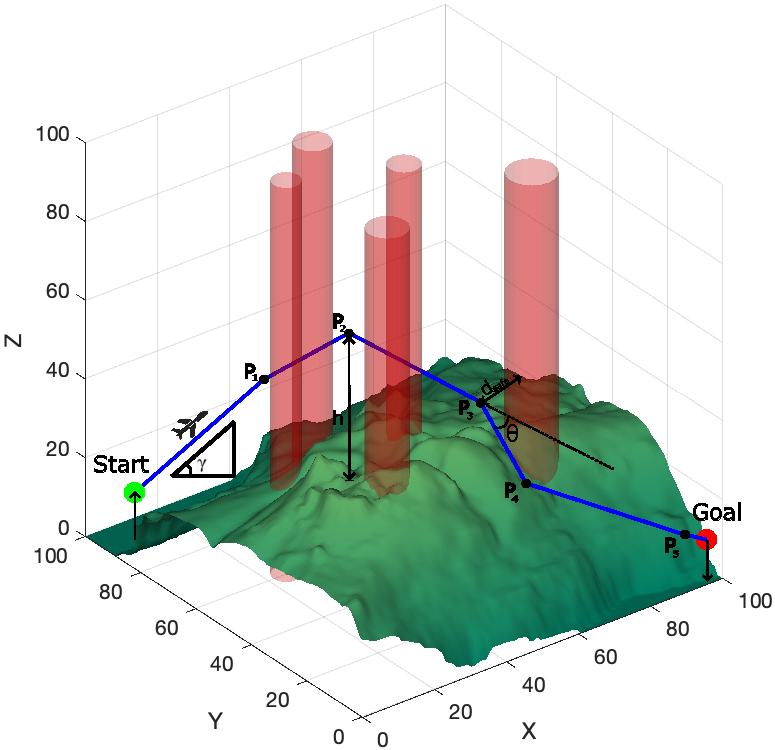
\includegraphics[width=\linewidth]{data/ProblemFormulation.pdf}
\caption{Geometric definition of UAV path planning parameters}
\label{fig:problem_formulation}
\end{figure}
A candidate path is encoded as a sequence of $n$ waypoints $P = [p_1, p_2, \ldots, p_n]$ where each $p_i = (x_i, y_i, z_i) \in \mathbb{R}^3$.
The UAV follows linear segments between consecutive waypoints, yielding total path length:
\begin{equation}
L(P) = \sum_{i=1}^{n-1} \|p_{i+1} - p_i\|_2
\label{eq:path_length}
\end{equation}
Path quality is evaluated through a weighted fitness function that balances competing objectives:
\begin{equation}
\begin{aligned}
f(P) ={}& \lambda_1 L(P) + \lambda_2 C_{\text{turn}}(P) + \lambda_3 C_{\text{climb}}(P) \\
&+ \lambda_4 C_{\text{alt}}(P) + C_{\text{safety}}(P)
\end{aligned}
\label{eq:fitness}
\end{equation}
The turn penalty $C_{\text{turn}}$ applies a linear penalty for directional changes that exceed a minimal tolerance threshold:
\begin{equation}
C_{\text{turn}}(P) = \sum_{i=2}^{n-1} \max\left(0, \theta_i - \theta_{\max}\right)
\end{equation}
where $\theta_i$ is the turn angle between consecutive segments $i-1$ and $i$, and $\theta_{\max}$ is the maximum zero-penalty turn threshold (set to $\symThetaTol$ rad).
The climb penalty $C_{\text{climb}}$ penalizes both steep climb adjustments and absolute climb angles:
\begin{equation}
\begin{aligned}
C_{\text{climb}}(P) = \sum_{i=2}^{n-1} \left( 2|\xi_i - \xi_{i-1}| + |\xi_i| + |\xi_{i-1}| \right)
\end{aligned}
\end{equation}
where $\xi_i = \arctan\left(\frac{z_{i+1} - z_i}{\|p_{i+1} - p_i\|_{xy}}\right)$ is the climb angle of the $i$-th segment. The safety penalty $C_{\text{safety}}$ acts as an absolute constraint combining terrain, obstacle, and path feasibility violations (applying infinite or heavy penalties for penetrating restricted boundaries):
\begin{equation}
\begin{aligned}
C_{\text{safety}}(P) = \sum_{i=1}^{n} \Bigl[ &\max(0, \mathcal{E}(x_i, y_i) + h_{\min} - z_i) \\
&+ \sum_{j=1}^{M} \max(0, r_j - d_{ij}) \Bigr]
\end{aligned}
\end{equation}
where $d_{ij}$ is the distance from waypoint $i$ to obstacle $j$.
The altitude cost $C_{\text{alt}}$ encourages the UAV to maintain low-level flight for terrain masking and energy efficiency:
\begin{equation}
C_{\text{alt}}(P) = \sum_{i=1}^{n} z_i
\end{equation}
The normalized weights $\lambda_1, \ldots, \lambda_4$ balance efficiency against soft constraints.
The safety term $C_{\text{safety}}$ dominates the objective to enforce strict feasibility.
Lower fitness values indicate better paths.

\section{Methods}
\label{sec:methods}
The RL based PSO parameter adaptation problem is formulated as a Markov Decision Process (MDP).
In the proposed algorithm, the MDP is defined by the tuple $(\mathcal{S}, \mathcal{A}, \mathcal{R}, \mathcal{T}, \symGamma)$ as illustrated in Figure~\ref{fig:mdp_components}.
The state space $\mathcal{S}$ encodes compact swarm statistics over a short temporal window.
The action space $\mathcal{A}$ is a $\symActiondim$-D latent control vector which is expanded into particle-wise PSO coefficients through the attractor-field parameter expansion.
The reward function $\mathcal{R}$ provides scale-invariant feedback from the relative improvement in global-best fitness.
The transition rules $\mathcal{T}$ describe deterministic updates computed via the standard PSO velocity and position equations, functioning effectively as the environment transition function during learning.
The discount factor $\symGamma$ determines the temporal preference for cumulative returns.
\begin{figure*}[!t]
\centering
\begin{tikzpicture}[
    x=1cm,
    y=1cm,
    >=Stealth,
    font=\normalsize,
    panel/.style={
        draw=black!35,
        thick,
        rounded corners=12pt,
        inner sep=10pt
    },
    box/.style={
        draw=black!65,
        thick,
        rounded corners=8pt,
        fill=white,
        align=center,
        inner sep=5pt,
        minimum height=2.2cm
    },
    smallbox/.style={
        draw=black!60,
        thick,
        rounded corners=7pt,
        fill=white,
        align=center,
        inner sep=4pt,
        minimum height=1.5cm
    },
    flow/.style={draw=black!80, line width=1.1pt, ->},
    train/.style={draw=red!70!black, line width=1.0pt, dashed, ->},
    faint/.style={draw=black!40, line width=0.9pt, ->},
    note/.style={
        draw=black!45,
        rounded corners=6pt,
        fill=yellow!12,
        align=center,
        font=\small,
        inner sep=4pt
    }
]

% Agent-side illustrations
\node[box, fill=blue!7, minimum width=3.4cm] (history) at (-6.1, 0.3) {%
\textbf{Swarm History}\\[-0.1em]
\begin{tikzpicture}[scale=0.8]
    \foreach \x/\f in {0.0/7,0.25/7,0.5/7,0.75/18} {
        \draw[draw=blue!45, fill=blue!\f] (\x,0) rectangle +(0.85,1.45);
        \foreach \yy in {0.18,0.36,...,1.26} {
            \draw[blue!55] (\x+0.08,\yy) -- (\x+0.77,\yy);
        }
    }
    \node[font=\scriptsize] at (0.95,-0.25) {$9$ features over $W=8$ steps};
\end{tikzpicture}};

\node[box, fill=blue!7, minimum width=3.4cm] (state) at (-1.7, 0.3) {%
\textbf{15D State Summary}\\[-0.2em]
\begin{tikzpicture}[scale=0.82]
    \foreach \i in {0,...,14} {
        \pgfmathsetmacro{\x}{mod(\i,5)*0.34}
        \pgfmathsetmacro{\y}{-floor(\i/5)*0.32}
        \draw[draw=blue!55, fill=blue!12] (\x,\y) rectangle +(0.27,0.22);
    }
    \node[font=\scriptsize] at (0.68,-1.15) {$[\,\text{current}_9,\ \text{mean}_{1:3},\ \text{trend}_{1:3}\,]$};
\end{tikzpicture}};

\node[box, fill=orange!10, minimum width=3.8cm] (sac) at (2.7, 0.3) {%
\textbf{SAC Controller}\\[-0.15em]
\begin{tikzpicture}[scale=0.82]
    \node[font=\scriptsize\bfseries, text=blue!70!black] at (0.95,0.9) {Actor};
    \foreach \y in {0.35,0.65,0.95} \fill[green!45!black] (0.0,\y) circle (1.8pt);
    \foreach \y in {0.25,0.55,0.85,1.15} \fill[gray!65] (0.75,\y) circle (1.8pt);
    \foreach \a in {0.25,0.55,0.85,1.15} \draw[gray!45] (0.02,0.35) -- (0.73,\a);
    \foreach \a in {0.25,0.55,0.85,1.15} \draw[gray!45] (0.02,0.65) -- (0.73,\a);
    \foreach \a in {0.25,0.55,0.85,1.15} \draw[gray!45] (0.02,0.95) -- (0.73,\a);
    \fill[orange!70] (1.45,0.7) circle (2.3pt);
    \foreach \a in {0.25,0.55,0.85,1.15} \draw[orange!60] (0.77,\a) -- (1.43,0.7);
    \node[font=\scriptsize\bfseries, text=red!70!black] at (0.95,-0.1) {Twin critics};
    \draw[draw=red!55, fill=red!10, rounded corners=3pt] (0.25,-0.55) rectangle +(0.5,0.28);
    \draw[draw=red!55, fill=red!10, rounded corners=3pt] (1.0,-0.55) rectangle +(0.5,0.28);
    \node[font=\scriptsize] at (0.95,-0.9) {target nets + entropy tuning};
\end{tikzpicture}};

\node[smallbox, fill=orange!14, minimum width=2.7cm] (action) at (6.0, 0.3) {%
\textbf{Latent Action}\\[-0.15em]
\begin{tikzpicture}[scale=0.85]
    \draw[draw=orange!70!black, fill=orange!18, rounded corners=8pt] (0,0) rectangle +(2.0,0.52);
    \foreach \i in {0,...,8} {
        \draw[orange!80!black] (0.12+0.2*\i,0.12) rectangle +(0.12,0.28);
    }
    \node[font=\scriptsize] at (1.0,-0.22) {$a_t \in [-1,1]^9$};
\end{tikzpicture}};

\node[note] (timing) at (8.8, 1.35) {observe / act every\\$n_t \approx T_{\max}/40$\\($25$ when $T_{\max}=1000$)};

\node[smallbox, fill=red!7, minimum width=2.9cm] (replay) at (8.3, -1.0) {%
\textbf{Replay Buffer}\\
\small training only};

% Environment-side illustrations
\node[smallbox, fill=yellow!12, minimum width=2.8cm] (reward) at (-7.0, -5.0) {%
\textbf{Relative Reward}\\[-0.1em]
\begin{tikzpicture}[scale=0.82]
    \draw[draw=yellow!55!black, fill=yellow!22, rounded corners=4pt] (0,0) rectangle +(1.7,0.42);
    \draw[green!55!black, line width=1.0pt] (0.12,0.12) -- (0.55,0.16) -- (0.9,0.26) -- (1.25,0.22) -- (1.58,0.32);
    \node[font=\scriptsize] at (0.85,-0.2) {$\mathcal{R}(f_{t-1},f_t)$};
\end{tikzpicture}};

\node[box, fill=green!8, minimum width=3.4cm] (eval) at (-2.6, -5.0) {%
\textbf{Fitness \& Swarm Stats}\\[-0.15em]
\begin{tikzpicture}[scale=0.82]
    \draw[draw=green!55!black, fill=green!10, rounded corners=5pt] (0,0) rectangle +(2.0,0.9);
    \node[font=\scriptsize] at (1.0,0.63) {$f_{\mathrm{gbest}}$, feasibility, diversity};
    \node[star, star points=5, star point ratio=2.1, fill=yellow!50, draw=orange!80, inner sep=1.1pt] at (0.26,0.28) {};
    \foreach \x/\y in {0.75/0.24,1.05/0.52,1.42/0.34,1.72/0.61}
        \fill[green!55!black] (\x,\y) circle (1.8pt);
    \node[font=\scriptsize] at (1.0,-0.16) {updates $pbest$ / $gbest$};
\end{tikzpicture}};

\node[box, fill=green!8, minimum width=4.0cm] (swarm) at (2.4, -5.0) {%
\textbf{PSO Search Step}\\[-0.15em]
\begin{tikzpicture}[scale=0.86]
    \node[star, star points=5, star point ratio=2.2, fill=yellow!50, draw=orange!80, inner sep=1.4pt] (g) at (2.15,0.72) {};
    \node[font=\scriptsize, above=1pt of g] {$gbest$};
    \foreach \p/\c/\tx/\ty/\dx/\dy in {
        p1/blue/0.15/0.18/0.58/0.28,
        p2/red/0.35/1.02/0.78/0.80,
        p3/purple/2.85/0.10/2.45/0.34,
        p4/green!50!black/2.95/1.00/2.52/0.82}
    {
        \fill[\c!55] (\tx,\ty) circle (1.8pt);
        \fill[\c!85] (\dx,\dy) circle (2.2pt);
        \draw[\c!75, line width=0.9pt, ->] (\tx,\ty) -- (\dx,\dy);
        \draw[\c!35, dashed] (\dx,\dy) -- (g);
    }
    \node[font=\scriptsize] at (1.5,-0.18) {apply $\{w_i,c_{1,i},c_{2,i}\}_{i=1}^N$};
\end{tikzpicture}};

\node[box, fill=orange!10, minimum width=3.5cm] (expand) at (6.7, -5.0) {%
\textbf{Attractor-Field Expansion}\\[-0.15em]
\begin{tikzpicture}[scale=0.85]
    \foreach \r in {0.25,0.5,0.75} \draw[orange!35] (0,0) circle (\r);
    \fill[orange!75] (0,0) circle (2.4pt);
    \node[font=\scriptsize\bfseries] at (0,0.28) {$a_t$};
    \draw[draw=blue!55, fill=blue!10, rounded corners=4pt] (0.55,0.55) rectangle +(1.0,0.22);
    \draw[draw=blue!55, fill=blue!10, rounded corners=4pt] (0.55,0.15) rectangle +(1.0,0.22);
    \draw[draw=blue!55, fill=blue!10, rounded corners=4pt] (0.55,-0.25) rectangle +(1.0,0.22);
    \node[font=\scriptsize] at (1.05,0.66) {$w_i$};
    \node[font=\scriptsize] at (1.05,0.26) {$c_{1,i}$};
    \node[font=\scriptsize] at (1.05,-0.14) {$c_{2,i}$};
    \draw[faint] (0.08,0.02) -- (0.55,0.66);
    \draw[faint] (0.08,0.00) -- (0.55,0.26);
    \draw[faint] (0.08,-0.02) -- (0.55,-0.14);
    \node[font=\scriptsize] at (0.72,-0.58) {particle-wise coefficients};
\end{tikzpicture}};

\node[smallbox, fill=yellow!10, minimum width=2.6cm] (context) at (9.25, -5.0) {%
\textbf{Context}\\
\small rank + geometry\\
modulation};

% Background panels
\begin{scope}[on background layer]
    \node[panel, fill=blue!4, fit=(history)(state)(sac)(action)(timing)(replay)] {};
    \node[font=\Large\bfseries] at (1.25,2.25) {Agent (Retained SAC Controller)};

    \node[panel, fill=green!4, fit=(reward)(eval)(swarm)(expand)(context)] {};
    \node[font=\Large\bfseries] at (1.15,-2.75) {Environment (PSO Search Process)};
\end{scope}

% Main loop
\draw[flow] (history) -- node[above, font=\small] {9 swarm features} (state);
\draw[flow] (state) -- node[above, font=\small] {$s_t \in \mathbb{R}^{15}$} (sac);
\draw[flow] (sac) -- node[above, font=\small] {policy output} (action);
\draw[flow] (action) -- node[right, font=\small] {$a_t \in \mathbb{R}^{9}$} (expand);
\draw[flow] (context) -- node[above, font=\small] {rank / geometry} (expand);
\draw[flow] (expand) -- node[above, font=\small] {$w_i,\ c_{1,i},\ c_{2,i}$} (swarm);
\draw[flow] (swarm) -- node[above, font=\small] {updated particles} (eval);
\draw[flow] (eval) -- node[above, font=\small] {next features} (history);
\draw[flow] (eval) -- node[above, font=\small] {$r_t$} (reward);

% Training-only loop
\draw[train] (state.south east) |- node[pos=0.28, right, font=\small] {training only} (replay.west);
\draw[train] (reward.north) |- (replay.west);
\draw[train] (action.south) |- (replay.north);
\draw[train] (replay.west) -- node[below, font=\small] {minibatch} (sac.east);

\end{tikzpicture}
\caption{Illustrative, repository-aligned MDP/data-flow view of the retained AFSACPSO configuration. The retained path builds nine swarm features over a temporal window, compresses them into a 15D state, maps that state to a 9D latent action with the SAC policy, and expands the latent action into particle-wise $(w_i,c_{1,i},c_{2,i})$ through the attractor-field module. The PSO environment then updates the swarm, evaluates the new global-best fitness, and returns both next-step swarm statistics and the relative-improvement reward. Dashed arrows denote training-only replay-buffer updates that are absent during frozen-policy deployment.}
\label{fig:mdp_components}
\end{figure*} 

\subsection{Reinforcement Learning Formulation}
Unless otherwise stated, the method described in this section refers to the retained attractor-field AFSACPSO configuration rather than the paper-aligned SAC-SAPSO compatibility branch.
To address the limitations of static state observations used in prior RL-PSO methods, we adopt a compact swarm-statistics state representation. This follows state-representation literature, which treats the state as a compact depiction of observations that preserves the information necessary for control and often benefits from temporal continuity or predictive dynamics \cite{Lesort2018State}.
At each iteration, the controller extracts nine normalized swarm-level features $f_1, \dots, f_9 \in [0,1]$ summarizing progress, diversity, fitness, constraints, and swarm kinematics. The exact mathematical formulation for each feature is detailed in Table~\ref{tab:state_features}.

\begin{table*}[htbp]
\centering
\small
\caption{Mathematical formulation of the 9 normalized swarm-level features }
\label{tab:state_features}
\renewcommand{\arraystretch}{1.3}
\begin{tabular}{llp{9.2cm}}
\hline
\textbf{Feature} & \textbf{Formula} & \textbf{Description} \\
\hline
$f_1$ Iteration progress & $t / \symMaxIters$ & Linear fraction of the search budget consumed. \\
$f_2$ Spatial diversity ratio & $\frac{1}{D} \sum_{d=1}^D \frac{\sigma(x_{\cdot,d})}{\Delta_d + \epsilon}$ & Average ratio of population standard deviation to bounding box span per dimension. \\
$f_3$ Elite fitness advantage & $\tanh\left(\symScaleElite \frac{\operatorname{median}(F) - \min(F)}{|\operatorname{median}(F)| + \epsilon}\right)$ & Normalized gap between median and best fitness, mapping large gaps asymptotically to 1. \\
$f_4$ Global stagnation & $\min\left(1, \frac{t - t_{\text{last\_improve}}}{\max(\symStagMinGlobal, \symStagRatioGlobal \symMaxIters)}\right)$ & Normalized iterations since the last global fitness improvement. \\
$f_5$ Feasibility-quality & $\symFeatWeightA \mu_{\text{feas}} + \symFeatWeightB \frac{1}{1 + \ln(1 + f_{\text{gbest}})}$ & Weighted combination of the feasible-particle ratio ($\mu_{\text{feas}}$) and log-scaled global best fitness. \\
$f_6$ Constraint-pressure & $\min(1, \mu_{\text{coll}} + P_{\text{terrain}} + P_{\text{danger}} + P_{\text{dup}})$ & Sum of collision ratio and log-scaled penalty averages ($P_k$) for terrain, danger zones, and duplicates. \\
$f_7$ Global-best attraction & $1 - \tanh\left(\frac{\frac{1}{\symPopsize}\sum_i \|x_i - g\|_2}{\bar{\Delta}\sqrt{D} + \epsilon}\right)$ & Inverse of the average distance to the global best relative to the expected bounding box diagonal. \\
$f_8$ Velocity alignment & $0.5 + 0.5 \left( \frac{1}{\symPopsize}\sum_i \frac{v_i \cdot (g - x_i)}{\|v_i\|_2 \|g - x_i\|_2 + \epsilon} \right)$ & Average cosine similarity between particle velocities and the direction to the global best. \\
$f_9$ Particle stagnation & $\frac{1}{\symPopsize} \sum_i \min\left( \frac{s_i}{\max(\symStagMinPart, \symStagRatioPart \symMaxIters)}, 1 \right)$ & Average normalized individual stagnation counter $s_i$ (iterations since personal best improved). \\
\hline
\end{tabular}
\end{table*}

These features are buffered over a temporal window of $\symWindowsize$ iterations.
In the retained benchmarked configuration, the deployed encoder is intentionally lightweight: it forms a $\symStatedim$-D state by concatenating the current nine features, the first three coordinates of the temporal mean, and the first three coordinates of the one-step trend.
This keeps the controller lightweight while still exposing short-horizon temporal context.
The nine base swarm features are clipped to $[0,1]$ before temporal aggregation; the appended trend terms in the final 15D state may be signed.
In the mathematical formulations detailed in Table~\ref{tab:state_features}, let $x_{i,d}$ and $v_{i}$ denote the position and velocity of particle $i$, $g$ the global best position, $F$ the set of valid particle fitnesses, $\symMaxIters$ the maximum iterations, $\symPopsize$ the swarm size, $D$ the problem dimension, and $\Delta_d = \max_i x_{i,d} - \min_i x_{i,d}$.
Table~\ref{tab:state_features} gives the retained feature design at the method level; the implementation uses fixed constants for the normalizers and weights in the corresponding code path.

The controller uses a scale-invariant relative improvement reward following \cite{vonEschwege2024Soft}. Let $f^{t-1}$ and $f^{t}$ denote the global best fitness before and after the PSO update at iteration $t$. The reward is:
\begin{equation}
r_t = \frac{2\left(f^{t-1} - f^{t}\right)}{\left|f^{t-1}\right| + \left|f^{t}\right| + \epsilon}
\label{eq:reward_total}
\end{equation}
where $\epsilon = 10^{-8}$ prevents division by zero.
This formulation is bounded in $[-2, 2]$, positive when fitness improves, negative when it worsens, and zero when unchanged. Because it normalizes by the absolute fitness values, the reward magnitude is consistent across functions with different fitness scales, which is essential for pretraining across diverse benchmark landscapes.

AFSACPSO employs Soft Actor-Critic \cite{Haarnoja2018Soft} to learn the parameter-adaptation policy.
The SAC objective is the entropy-regularized expected return:
\begin{equation}
J(\pi) = \mathbb{E}_{\tau \sim \pi}\left[\sum_{t=0}^{T} \gamma^t \left(r_t + \alpha \mathcal{H}(\pi(\cdot|\mathbf{s}_t))\right)\right]
\label{eq:sac_objective}
\end{equation} where $\alpha$ is the temperature parameter (automatically tuned) and $\mathcal{H}$ is the policy entropy.
The algorithm maintains three components: Actor Network $\pi_\theta(\mathbf{a}|\mathbf{s})$: A Gaussian policy with learnable mean and diagonal covariance. In the retained implementation the actor is a compact MLP operating on the flat 15D state vector. Actions are sampled via reparameterization:
\begin{equation}
\mathbf{a}_t = \tanh(\boldsymbol{\mu}_\theta(\mathbf{s}_t) + \boldsymbol{\sigma}_\theta(\mathbf{s}_t) \odot \boldsymbol{\epsilon}), \quad \boldsymbol{\epsilon} \sim \mathcal{N}(0, \mathbf{I})
\end{equation} Twin Critic Networks $Q_{\phi_1}, Q_{\phi_2}$: Two independent scalar Q-functions are retained together with target networks. The critic loss minimizes the Bellman error using the minimum of both critics:
\begin{equation}
\begin{aligned}
L_Q(\phi_i) = \mathbb{E}_{(\mathbf{s},\mathbf{a},r,\mathbf{s}')} \Bigl[ \bigl(Q_{\phi_i}(\mathbf{s}, \mathbf{a}) - (&r + \symGamma \min_{j=1,2} Q_{\phi_j}(\mathbf{s}', \mathbf{a}') \\
&- \alpha \log \pi_\theta(\mathbf{a}'|\mathbf{s}') )\bigr)^2 \Bigr]
\end{aligned}
\end{equation} Temperature Parameter $\alpha$: Automatically adjusted to match a target entropy $\bar{\mathcal{H}} = -\dim(\mathcal{A}) = -\symActiondim$ via:
\begin{equation}
L_\alpha = \mathbb{E}_{\mathbf{s} \sim \mathcal{D}}\left[-\alpha \left(\log \pi_\theta(\mathbf{a}|\mathbf{s}) + \bar{\mathcal{H}}\right)\right]
\end{equation} In the retained configuration, the controller uses standard SAC with twin scalar critics, target networks, and automatic entropy tuning.
During deployment, only the actor is used (critics are discarded) and no gradient updates occur.

\subsection{Attractor-Field Parameter Expansion}
The attractor-field parameter expansion is the core mechanism linking the SAC controller to particle-wise PSO adaptation.
Like per-particle adaptive PSO schemes such as SAEPSO and UAPSO \cite{Liu2025A, Isiet2019Selfadapting}, the expansion conditions each particle's coefficients on its current search status.
However, instead of hand-crafting the coefficient rules directly, AFSACPSO learns a shared latent control vector $\mathbf{a}_t = [a_1,\dots,a_9]^\top \in [-1,1]^9$ and expands it into particle-wise PSO coefficients through a combination of population-level control and rank-normalized geometric context signals.

For each particle $i$, three geometric signals are computed from the particle's relationship to its PSO attractors:
\begin{equation}
\begin{aligned}
\tau_{i,t} &= \frac{\|x_i - g\|_2 - \|x_i - p_i\|_2}{\|x_i - g\|_2 + \|x_i - p_i\|_2 + \epsilon}, \\
\alpha_{i,t} &= \frac{v_i \cdot (g - x_i)}{\|v_i\|_2 \, \|g - x_i\|_2 + \epsilon}, \\
\delta_{i,t} &= \frac{f(x_i) - f(p_i)}{|f(p_i)| + 1},
\end{aligned}
\label{eq:rank_residual_context}
\end{equation}
where $p_i$ is the personal best position of particle~$i$, $g$ is the global best position, and $f$ denotes fitness.
The attractor tension $\tau$ measures whether a particle is closer to the global or personal best, the velocity alignment $\alpha$ captures how well the particle's current velocity is directed toward the global best, and the fitness drift $\delta$ quantifies how much the current fitness has degraded from the personal best.
All three raw signals are rank-normalized across the swarm to $[-0.5, +0.5]$, yielding centered values $\hat{\tau}_{i,t}$, $\hat{\alpha}_{i,t}$, and $\hat{\delta}_{i,t}$.
This rank normalization prevents signal collapse near convergence and ensures comparable scales regardless of the fitness landscape.

The latent action is split into population-level bias and per-particle modulation.
Actions $a_1, a_4, a_7$ are mapped from $[-1,1]$ to $[0,1]$ to control the population-level parameter setting, while the remaining actions modulate the geometric signals with a spread constant $\symSpread$:
\begin{equation}
\begin{aligned}
\ell_{w} &= \tfrac{a_1 + 1}{2}, &\quad
m_{w,i} &= \symSpread\!\left(a_2\,\hat{\alpha}_{i,t} + a_3\,\hat{\tau}_{i,t}\right), \\
\ell_{c_1} &= \tfrac{a_4 + 1}{2}, &\quad
m_{c_1,i} &= \symSpread\!\left(a_5\,\hat{\delta}_{i,t} + a_6\,\hat{\tau}_{i,t}\right), \\
\ell_{c_2} &= \tfrac{a_7 + 1}{2}, &\quad
m_{c_2,i} &= \symSpread\!\left({-a_8}\,\hat{\tau}_{i,t} - a_9\,\hat{\alpha}_{i,t}\right),
\end{aligned}
\label{eq:rank_residual_delta}
\end{equation}
and the final PSO coefficients are obtained by mapping to the admissible ranges
\begin{equation}
\begin{aligned}
w_{i,t} &= \symWclipMin + (\symWclipMax - \symWclipMin)\,\operatorname{clip}_{[0,\,1]}\!\left(\ell_{w} + m_{w,i}\right), \\
c_{1,i,t} &= \symCclipMin + (\symCclipMax - \symCclipMin)\,\operatorname{clip}_{[0,\,1]}\!\left(\ell_{c_1} + m_{c_1,i}\right), \\
c_{2,i,t} &= \symCclipMin + (\symCclipMax - \symCclipMin)\,\operatorname{clip}_{[0,\,1]}\!\left(\ell_{c_2} + m_{c_2,i}\right).
\end{aligned}
\label{eq:rank_residual_final}
\end{equation}
This design preserves a low-dimensional RL control problem while still allowing heterogeneous parameter assignments across the swarm.
Particles that are drifting away from their personal best or poorly aligned with the global best direction can be pushed toward more exploratory settings, while particles with strong attractor alignment remain closer to exploitative coefficients.
The mapping keeps the controller compact and avoids the dimensionality explosion that would arise if the policy directly emitted all $3\symPopsize$ particle parameters independently.

\subsection{Algorithm Workflow}
AFSACPSO operates in two phases: an offline pretraining phase that builds a general parameter-adaptation policy, and a deployment phase that applies the frozen policy to the target optimization problem.

\paragraph{Phase 1: Pretraining on benchmark functions.}
Following the protocol of \cite{vonEschwege2024Soft}, the SAC agent is trained across a suite of 45 standard 30-dimensional minimization functions drawn from the global optimization literature, following the same train/test split as in Table 3 of \cite{vonEschwege2024Soft}.
Each training episode selects a function from the training set, initializes a fresh swarm, and runs PSO for $T_{\text{pre}}$ iterations while the agent collects transitions and updates its policy.
After cycling through the training set, the agent has accumulated experience across diverse fitness landscapes, learning a general policy for when to favor exploration versus exploitation based on swarm state alone.
In the offline pretraining configuration, the PSO settings are aligned with deployment: swarm size 100, iteration budget 1000, and observation interval 25, yielding 40 control decisions and 40 gradient updates per episode.
The SAC hyperparameters for this offline pretraining configuration follow \cite{vonEschwege2024Soft}: discount $\gamma=1$, target smoothing $\tau=0.005$, actor and critic networks with two hidden layers of 256 units each, replay buffer size $10^6$, and $2\times10^5$ total gradient steps over 5000 episodes.

\paragraph{Phase 2: Frozen-policy deployment.}
Once pretrained, the actor weights are frozen (no further gradient updates) and the policy is deployed on the target problem.
In the retained benchmarked configuration, the controller refreshes its observation and latent action every 25 PSO iterations, while reusing the most recent expanded coefficients between observation points.
At each observation step, the controller encodes the compact swarm state, produces a 9D latent action, and expands it through the attractor-field parameter expansion into particle-wise PSO coefficients.
Because the policy was trained on diverse landscapes, it generalizes to unseen fitness functions---including UAV path planning---without additional online learning.
Algorithm~\ref{alg:apexpso} summarizes the deployment-phase loop.

\begin{algorithm}[H]
\caption{AFSACPSO Deployment (Frozen Policy)}
\label{alg:apexpso}
\begin{algorithmic}[1]
\State \textbf{Input:} Swarm size $\symPopsize$, max iterations $\symMaxIters$, pretrained actor $\pi_\theta$
\State \textbf{Initialize:} Swarm positions $x_i^0$, velocities $v_i^0$, personal bests $p_i^0$, global best $g^0$, observation interval $n_t$
\State Encode the initial swarm state and query $\pi_\theta$ once to obtain the initial expanded coefficients
\For{$t = 1$ to $\symMaxIters$}
\If{$t$ is an observation step or $t=\symMaxIters$}
\State Compute compact swarm statistics $s_t$
\State Sample latent action $\mathbf{a}_t \sim \pi_\theta(\cdot|s_t)$ \Comment{No gradient updates}
\State Expand $\mathbf{a}_t$ through the attractor-field parameter expansion to particle-wise PSO coefficients $\{w_{i,t}, c_{1,i,t}, c_{2,i,t}\}_{i=1}^{\symPopsize}$
\EndIf
\For{each particle $i \in \{1, \dots, \symPopsize\}$}
\State Update velocity $v_i^{t} \leftarrow w_{i,t} v_i^{t-1} + c_{1,i,t} r_1 (p_i^{t-1} - x_i^{t-1}) + c_{2,i,t} r_2 (g^{t-1} - x_i^{t-1})$
\State Update position $x_i^{t} \leftarrow x_i^{t-1} + v_i^{t}$
\EndFor
\State Evaluate fitness $f(x_i^t)$ and update $p_i^t$ and $g^t$
\EndFor
\State \Return Optimal solution $g^t$
\end{algorithmic}
\end{algorithm}

\section{Experimental Setup}
\label{sec:experimental_setup}
Path quality is measured by global best fitness (Equation \ref{eq:fitness}), which combines path length, turning penalties, climbing penalties, and collision penalties.
Lower fitness indicates better paths.
The main benchmark evaluates the retained AFSACPSO configuration in attractor-field mode (9D latent action) against RL-based and classical PSO baselines.
All compared methods use the same UAV scenarios, a swarm size of 100 particles, a maximum budget of 1,000 iterations per run, and a common base seed ($1000r + 100s$ for run $r$ and scenario $s$) to ensure paired statistical comparison under matched stochastic conditions.

The evaluation is organized into two stages: offline pretraining of the SAC controller, followed by frozen-policy UAV path-planning evaluation.
The AFSACPSO controller is pretrained on 45 standard 30-dimensional benchmark functions, following the same train/test split as in Table 3 of \cite{vonEschwege2024Soft}, with the remaining 7 functions held out for generalisation checks.
Pretraining runs for 5,000 episodes with one transition recorded every 25 iterations, yielding $2\times 10^5$ gradient steps.
SAC hyperparameters follow \cite{vonEschwege2024Soft}: $\gamma=1$, $\tau=0.005$, two hidden layers of 256 units, replay buffer $10^6$, and batch size 256.

After offline training, the actor weights are frozen and no further gradient updates are performed during UAV path planning.
At deployment, the 9D latent action is expanded into particle-wise PSO coefficients $w_{i} \in [0.1, 0.9]$, $c_{1,i} \in [0.5, 2.5]$, and $c_{2,i} \in [0.5, 2.5]$ via the attractor-field parameter expansion.
The frozen controller is compared against two benchmark groups:
\begin{enumerate}
    \item \textbf{RL-based baselines:} RLAM-PSO (DDPG) \cite{Yin2023RLAMPSO}, DQN-PSO \cite{Aoun2024Deep}, SAC-SAPSO \cite{vonEschwege2024Soft}, MPSORL \cite{Meng2023Multistrategy}, and PPO-PSO \cite{Klein2024Optimizing}.
    \item \textbf{Classical and adaptive PSO baselines:} PSO-Standard, PSO-LDIW, FIPS, CLPSO, SAEPSO, SAEPSO*, and UAPSO.
\end{enumerate}
For each algorithm, we conduct 30 independent runs per scenario.
Inferential analysis uses two-sided paired t-tests (primary) and two-sided Wilcoxon signed-rank tests (robustness), with Holm--Bonferroni correction applied to all pairwise p-values within each scenario.
All results reported in Tables~\ref{tab:rl_comparison} and \ref{tab:others_comparison} follow this protocol.




\section{Results}
\label{sec:results}

\subsection{Offline Pretraining Results}
Table~\ref{tab:offline_pretraining_logs} summarizes the retained offline pretraining logs for six controller variants stored in the repository: RLAMPSO, the attractor-field AFSACPSO controller, matched global and fixed 5-subgroup SAC controllers, a direct per-particle SAC controller, and the paper-aligned SAC-SAPSO-style global controller.
Because consecutive pretraining episodes optimize different benchmark functions with heterogeneous objective scales, raw episode fitness is not used here as a comparative metric.
Instead, we report protocol-level and implementation-level quantities that are directly comparable across models, together with a held-out deployment summary on the seven benchmark test functions.
The held-out benchmark uses the frozen pretrained models directly with 100 particles, 1{,}000 PSO iterations, and 30 independent runs per function; the reported mean and standard deviation aggregate the resulting 210 held-out trials per variant.
All six retained models complete the full 5{,}000-episode pretraining budget without non-finite saved weights. RLAMPSO does not expose an SAC entropy coefficient because it is a DDPG-based controller rather than a SAC-based one.

The table highlights the main computational tradeoff of the retained controller family.
All SAC-based variants are trained for the same 5{,}000-episode budget, so the dominant differences arise from action-space size and model capacity rather than from training duration.
The per-particle controller is by far the largest SAC model, with 224{,}088 actor parameters and a 300-dimensional action space, and correspondingly incurs the highest SAC-side computational cost at 13.80\,h CPU time.
By contrast, the retained attractor-field controller uses a 9-dimensional action space and 74{,}514 actor parameters, placing it much closer to the global and 5-subgroup variants than to the direct per-particle controller.
RLAMPSO remains the most expensive controller overall in the retained artifacts, requiring 15.92\,h CPU time despite a smaller actor parameter count than several SAC variants.
Among the SAC-based variants, the saved final entropy coefficient is smallest for the per-particle controller ($4.54\times 10^{-5}$), followed by the attractor-field controller ($4.49\times 10^{-4}$) and the matched global controller ($9.55\times 10^{-4}$), while the 5-subgroup controller retains a larger value (0.0191) and the paper-aligned SAC-SAPSO variant remains much higher (2.7183).
On the held-out benchmark, RLAMPSO attains the lowest aggregate mean ($-7.62 \pm 17.17$), followed by the fixed 5-subgroup controller ($-7.20 \pm 16.38$), the retained attractor-field controller ($-7.13 \pm 16.23$), and the matched global controller ($-7.04 \pm 15.95$).
The held-out deployment CPU times still reveal a clear efficiency gap: RLAMPSO requires 746.70\,s across the full seven-function, 30-run evaluation, whereas the SAC-based variants remain between 185.79\,s and 249.41\,s.
At the function level, the attractor-field controller wins on 6 of 7 held-out functions against the direct per-particle SAC controller, 7 of 7 against SAC-SAPSO, 4 of 7 against RLAMPSO, and 3 of 7 against both the matched global and fixed 5-subgroup SAC controllers.
These results indicate that the retained attractor-field mapping is competitive but not uniquely dominant on the held-out benchmark suite; its retention is therefore justified primarily by the downstream UAV benchmark, while the held-out wins suggest that the main advantage of attractor-field control is consistency against simpler or less structured control interfaces rather than universal dominance on pooled mean fitness.

\begin{table*}[!t]
\centering
\small
\caption{Offline pretraining protocol and held-out benchmark summary for retained pretrained models in the repository. All variants are trained for 5{,}000 episodes on the same 45-function benchmark suite with 100 particles and 1{,}000 PSO iterations per episode. The held-out benchmark evaluates the frozen pretrained models on the seven test functions using the same 100-particle, 1{,}000-iteration PSO budget and 30 runs per function. Actor params denotes the number of trainable parameters in the policy network used to generate PSO-control actions.}
\label{tab:offline_pretraining_logs}
\resizebox{\textwidth}{!}{%
\begin{tabular}{lcccccc}
\hline
Variant & Action dim. & Actor params & Pretrain Time (h) & Final $\alpha$ & Test Time (s) & Wins$^\dagger$ \\
\hline
RLAMPSO \cite{Yin2023RLAMPSO} & 20 & \textbf{10644} & 15.92 & --- & 746.70 & 4 \\
Attractor-field & 9 & 74514 & 8.15 & $4.49\times10^{-4}$ & 249.41 & --- \\
Global & \textbf{3} & 71430 & \textbf{7.96} & $9.55\times10^{-4}$ & 201.76 & 3 \\
5-subgroup  & 15 & 77598 & 11.40 & $1.91\times10^{-2}$ & 199.23 & 3 \\
Per-particle & 300 & 224088 & 13.80 & $4.54\times10^{-5}$ & \textbf{185.79} & 6 \\
SAC-SAPSO \cite{vonEschwege2024Soft} & \textbf{3} & 93958 & 8.95 & $2.72$ & 201.45 & 7 \\
\hline
\end{tabular}}
\vspace{2pt}

\raggedright\footnotesize{$^\dagger$Wins for the attractor-field controller over the 7 held-out functions, ordered as Global/5Sub/PerParticle/RLAMPSO/SAC-SAPSO. Lower mean fitness wins per function.}
\end{table*}

\subsection{Comparison Against RL-Based Baselines}
Table~\ref{tab:rl_comparison} summarizes the comparison against RL based baselines, while Figures~\ref{fig:rl_3d_grid}--\ref{fig:rl_diagnostics} show representative trajectory and diagnostic panels for the four scenario RL benchmark.
For this external comparison, we use SACPSO-Global rather than AFSACPSO, because the internal same-backbone ablation identifies it as the strongest retained frozen deployment variant under the shared 15D state representation and SAC pretraining pipeline.
In the current benchmark, SACPSO-Global achieves the lowest mean fitness in Scenarios 1 and 3 (1569.32 and 1500.78), while MPSORL attains the best mean fitness in Scenarios 2 and 4 (1554.99 and 12258.77).
SACPSO-Global remains close to MPSORL in those two scenarios and records lower mean fitness than RLAMPSO, DQN-PSO, SAC-SAPSO, and PPO-PSO in all four cases.
DQN-PSO deteriorates sharply as scenario complexity increases, producing the largest variance in Scenarios 2, 3, and 4.
Holm-corrected paired tests show that SACPSO-Global significantly outperforms RLAMPSO and SAC-SAPSO in all four scenarios, and significantly outperforms DQN-PSO in Scenarios 2, 3, and 4 while remaining directionally better in Scenario 1.
Against PPO-PSO, SACPSO-Global is directionally better in Scenarios 1, 2, and 3 and significantly better in Scenario 4.
Against MPSORL, SACPSO-Global is directionally better in Scenarios 1 and 3 and directionally worse in Scenarios 2 and 4, with no significant difference after Holm correction in the latter three cases.
PPO-PSO is a baseline inspired by the iSOMA-RL framework of Klein et al.\ \cite{Klein2024Optimizing}, which applies Proximal Policy Optimization to dynamically adapt swarm intelligence parameters; we adapt their PPO-based online control scheme to PSO, replacing iSOMA-specific parameters with the PSO velocity-update coefficients $(\omega, c_1, c_2)$ and using a continuous action space following Schulman et al.\ \cite{Schulman2017Proximal}.
In the representative convergence plot of Figure~\ref{fig:rl_diagnostics}, PPO-PSO descends fastest and reaches the lowest final fitness, while the retained SAC variant converges more gradually and finishes in the same broad band as the strongest RL baselines.
The reward panel shows that PPO-PSO and MPSORL maintain more consistently positive smoothed rewards, whereas the retained SAC controller exhibits a more oscillatory trace with a long negative phase early in the run and mixed reward thereafter.
The parameter-tracking panel provides direct evidence that the retained SAC controller uses a wide adaptive range for $w$, $c_1$, and $c_2$, unlike the flatter PPO-PSO trace and the more step-like SAC-SAPSO and MPSORL traces.
The trajectory panels in Figures~\ref{fig:rl_3d_grid} and \ref{fig:rl_topview_grid} show several distinct feasible route families rather than a single visually dominant path, which is consistent with the table-level result that SACPSO-Global is the strongest retained frozen SAC deployment variant against RLAMPSO, DQN-PSO, SAC-SAPSO, and PPO-PSO in this rerun, while remaining statistically tied with MPSORL on the harder scenarios.
\begin{table*}[!t]
\centering
\small
\resizebox{\textwidth}{!}{%
\begin{tabular}{lccc ccc ccc ccc}
\hline
\multirow{2}{*}{Algorithm} & \multicolumn{3}{c}{Scenario 1} & \multicolumn{3}{c}{Scenario 2} & \multicolumn{3}{c}{Scenario 3} & \multicolumn{3}{c}{Scenario 4} \\
\cline{2-13}
 & Fitness & Time & TTest & Fitness & Time & TTest & Fitness & Time & TTest & Fitness & Time & TTest \\
\hline
RLAMPSO\cite{Yin2023RLAMPSO} & 1680.11 $\pm$ 43.35 & 92.52 & $\uparrow\uparrow$ & 1754.73 $\pm$ 95.19 & 67.17 & $\uparrow\uparrow$ & 1791.23 $\pm$ 76.81 & 65.51 & $\uparrow\uparrow$ & 12686.66 $\pm$ 206.94 & 109.74 & $\uparrow\uparrow$ \\
DQN-PSO\cite{Aoun2024Deep} & 1644.71 $\pm$ 73.36 & 126.85 & $\uparrow$ & 1707.62 $\pm$ 191.52 & 109.22 & $\uparrow\uparrow$ & 1891.45 $\pm$ 302.62 & 110.22 & $\uparrow\uparrow$ & 12558.21 $\pm$ 319.93 & 151.76 & $\uparrow\uparrow$ \\
SAC-SAPSO \cite{vonEschwege2024Soft} & 1767.65 $\pm$ 116.00 & 37.07 & $\uparrow\uparrow$ & 1811.86 $\pm$ 164.13 & 33.47 & $\uparrow\uparrow$ & 1915.42 $\pm$ 203.58 & 35.50 & $\uparrow\uparrow$ & 12879.02 $\pm$ 351.80 & 71.54 & $\uparrow\uparrow$ \\
PPO-PSO \cite{Klein2024Optimizing} & 1698.23 $\pm$ 252.71 & 55.89 & $\uparrow$ & 1620.04 $\pm$ 92.61 & 44.37 & $\uparrow$ & 1587.71 $\pm$ 149.50 & 47.33 & $\uparrow$ & 12568.22 $\pm$ 332.97 & 85.17 & $\uparrow\uparrow$ \\
MPSORL \cite{Meng2023Multistrategy} & 1631.49 $\pm$ 81.03 & 33.77 & $\uparrow$ & \textbf{1554.99} $\pm$ 103.22 & 32.61 & $\downarrow$ & \textbf{1505.15} $\pm$ 93.52 & 34.17 & $\downarrow$ & \textbf{12258.77} $\pm$ 138.96 & 71.04 & $\downarrow$ \\
SACPSO-Global & 1569.32 $\pm$ 101.20 & 39.57 & --- & 1557.72 $\pm$ 102.72 & 35.27 & --- & 1500.78 $\pm$ 112.27 & 36.14 & --- & 12325.72 $\pm$ 170.05 & 77.10 & --- \\
\hline
\end{tabular}%
}
\caption{Performance comparison of RL based PSO parameter adaptation algorithms across the four scenario RL benchmark. SACPSO-Global is included as the strongest retained frozen deployment variant from the internal same-backbone ablation, while AFSACPSO is analyzed separately as the proposed control-interface study in Table~\ref{tab:sac_granularity_ablation}. Fitness reports Mean $\pm$ Standard Deviation over 30 runs. Time reports mean total planning time per run in seconds. TTest compares each method against SACPSO-Global using Holm-corrected paired t-tests, where $\downarrow\downarrow$ = significantly better, $\uparrow\uparrow$ = significantly worse, $\downarrow$ = better but not significant, and $\uparrow$ = worse but not significant.}
\label{tab:rl_comparison}
\end{table*}

\begin{figure*}[!t]
\centering
\begin{subfigure}{0.24\textwidth}
\centering

\includegraphics[width=\linewidth,height=0.16\textheight,keepaspectratio]{data/rlbased/Scenario1_3D.pdf}
\caption{Scenario 1}
\end{subfigure}
\hfill
\begin{subfigure}{0.24\textwidth}
\centering

\includegraphics[width=\linewidth,height=0.16\textheight,keepaspectratio]{data/rlbased/Scenario2_3D.pdf}
\caption{Scenario 2}
\end{subfigure}
\hfill
\begin{subfigure}{0.24\textwidth}
\centering

\includegraphics[width=\linewidth,height=0.16\textheight,keepaspectratio]{data/rlbased/Scenario3_3D.pdf}
\caption{Scenario 3}
\end{subfigure}
\hfill
\begin{subfigure}{0.24\textwidth}
\centering

\includegraphics[width=\linewidth,height=0.16\textheight,keepaspectratio]{data/rlbased/Scenario4_3D.pdf}
\caption{Scenario 4}
\end{subfigure}
\caption{RL based 3D trajectory comparisons across the four benchmark scenarios.}
\label{fig:rl_3d_grid}
\end{figure*}

\begin{figure*}[!t]
\centering
\begin{subfigure}{0.24\textwidth}
\centering

\includegraphics[width=\linewidth,height=0.16\textheight,keepaspectratio]{data/rlbased/Scenario1_TopView.pdf}
\caption{Scenario 1}
\end{subfigure}
\hfill
\begin{subfigure}{0.24\textwidth}
\centering

\includegraphics[width=\linewidth,height=0.16\textheight,keepaspectratio]{data/rlbased/Scenario2_TopView.pdf}
\caption{Scenario 2}
\end{subfigure}
\hfill
\begin{subfigure}{0.24\textwidth}
\centering

\includegraphics[width=\linewidth,height=0.16\textheight,keepaspectratio]{data/rlbased/Scenario3_TopView.pdf}
\caption{Scenario 3}
\end{subfigure}
\hfill
\begin{subfigure}{0.24\textwidth}
\centering

\includegraphics[width=\linewidth,height=0.16\textheight,keepaspectratio]{data/rlbased/Scenario4_TopView.pdf}
\caption{Scenario 4}
\end{subfigure}
\caption{RL based top-view trajectory comparisons across the four benchmark scenarios.}
\label{fig:rl_topview_grid}
\end{figure*}

\begin{figure*}[!t]
\centering
\begin{subfigure}{0.32\textwidth}
\centering

\includegraphics[width=\linewidth,height=0.18\textheight,keepaspectratio]{data/rlbased/Convergence_Comparison.pdf}
\caption{Convergence}
\end{subfigure}
\hfill
\begin{subfigure}{0.32\textwidth}
\centering
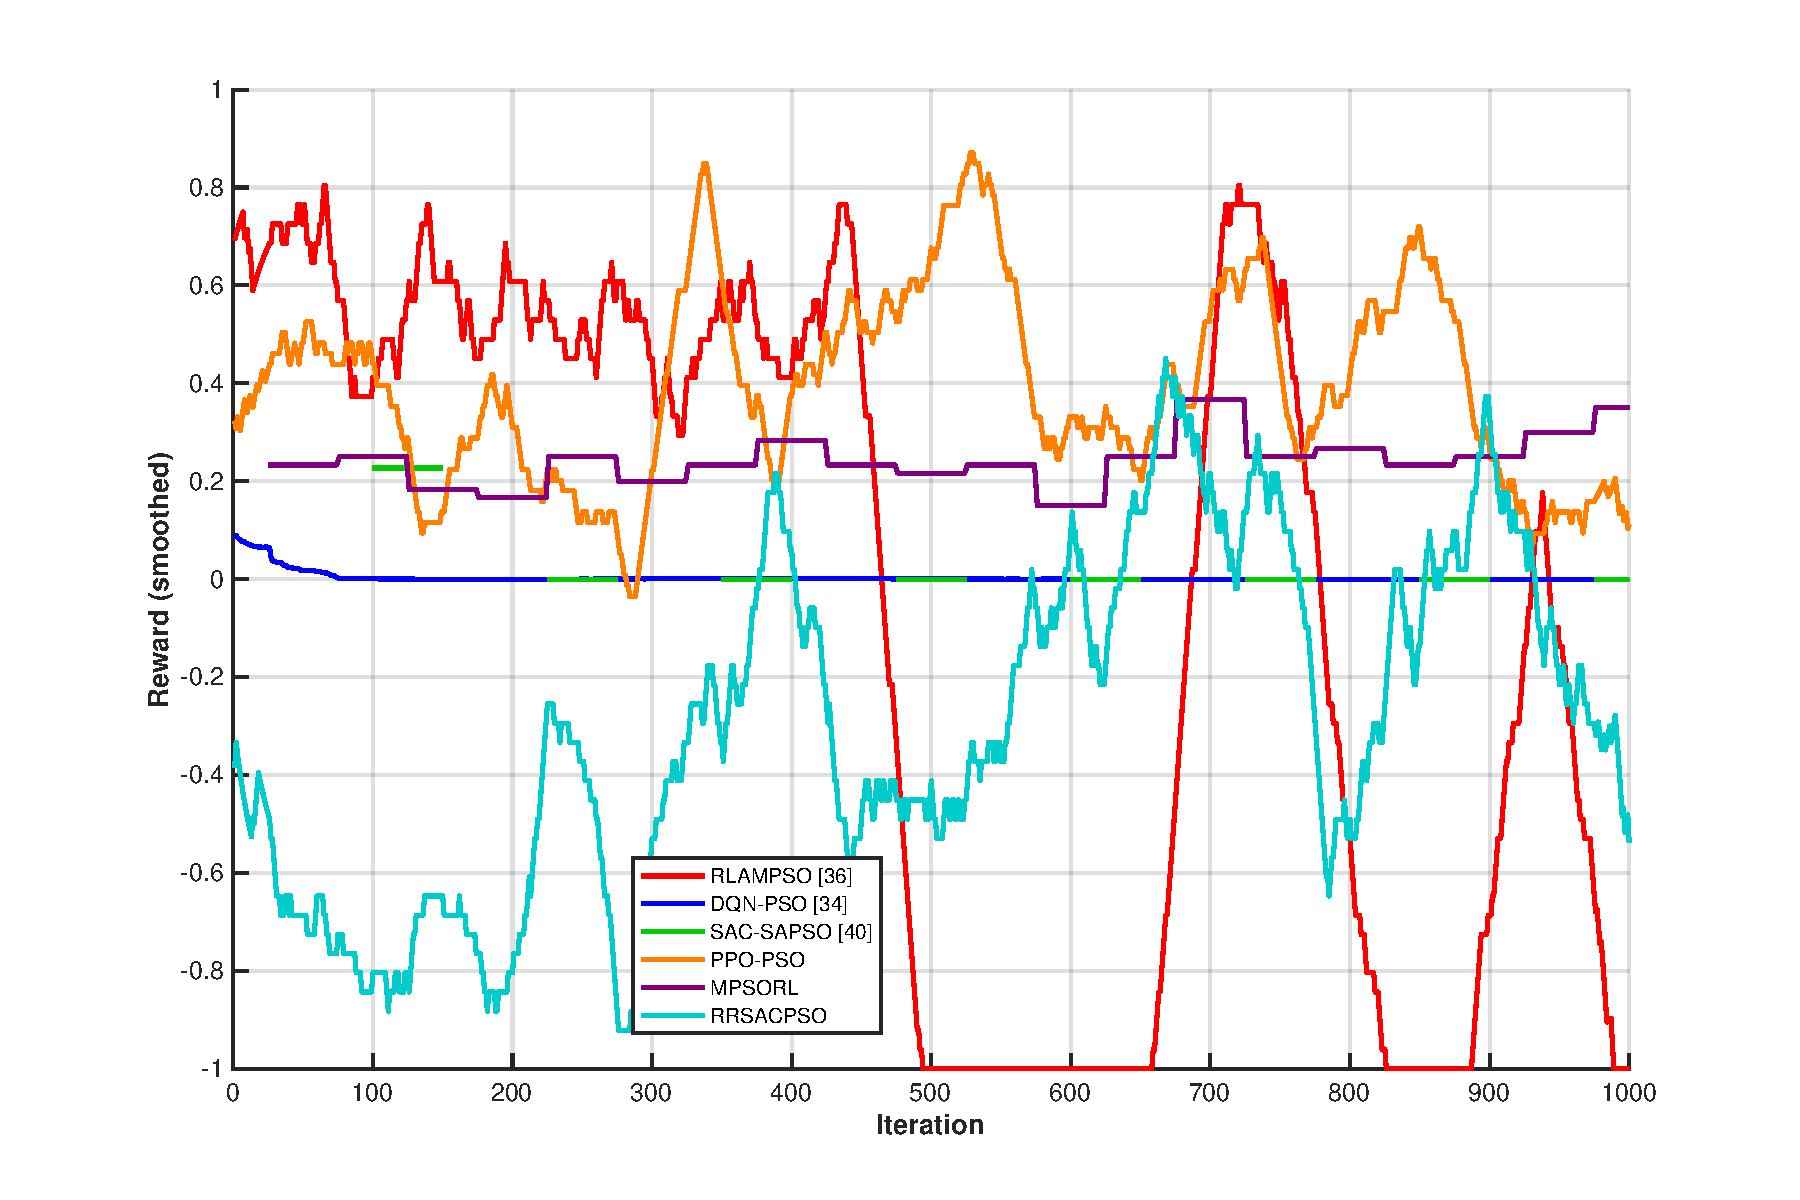
\includegraphics[width=\linewidth,height=0.18\textheight,keepaspectratio]{data/rlbased/Reward_Comparison.pdf}
\caption{Reward}
\end{subfigure}
\hfill
\begin{subfigure}{0.32\textwidth}
\centering

\includegraphics[width=\linewidth,height=0.18\textheight,keepaspectratio]{data/rlbased/Parameter_Tracking.pdf}
\caption{Parameter tracking}
\end{subfigure}
\caption{RL based convergence, reward, and parameter-tracking diagnostics.}
\label{fig:rl_diagnostics}
\end{figure*}
\subsection{Comparison Against Classical and Adaptive PSO Baselines}
Table~\ref{tab:others_comparison} summarizes the comparison against classical and adaptive PSO baselines, while Figures~\ref{fig:others_3d_grid}--\ref{fig:others_convergence_tracking} show the corresponding representative trajectory and diagnostic panels for the four scenario benchmark.
Within this comparison, SAEPSO achieves the lowest mean fitness in Scenarios 1 and 4, while SAEPSO* is best in Scenarios 2 and 3.
As in Table~\ref{tab:rl_comparison}, the SAC row here is SACPSO-Global, i.e., the strongest retained frozen deployment variant identified by the internal ablation.
SACPSO-Global attains lower mean fitness than PSO-Standard, FIPS, CLPSO, and UAPSO in all four scenarios, while SAEPSO, SAEPSO*, and PSO-LDIW achieve equal or lower mean fitness in at least one scenario.
Holm-corrected paired tests show that SACPSO-Global is significantly worse than SAEPSO in Scenarios 1 and 4 and worse than SAEPSO* in Scenario 4.
It remains statistically indistinguishable from PSO-LDIW across all four scenarios and from SAEPSO* in Scenarios 1--3.
It significantly outperforms CLPSO in all four scenarios, with additional significant gains over FIPS in Scenarios 1, 2, and 4 and over UAPSO in Scenario 4.
In the representative convergence panel of Figure~\ref{fig:others_convergence_tracking}, SAEPSO and SAEPSO* finish lowest, while the retained SAC deployment variant remains in the leading group but does not end below the strongest classical baselines.
The parameter-tracking panel shows that the retained SAC controller follows a markedly more variable coefficient profile than PSO-LDIW and UAPSO, whose schedules are much smoother and more prescribed.
The 3D and top-view trajectory panels again show multiple feasible route families rather than clear visual dominance by any single method, which matches the quantitative result that SACPSO-Global is competitive but not superior to the strongest SAEPSO-family baselines.
\begin{table*}[!t]
\centering
\small
\resizebox{\textwidth}{!}{%
\begin{tabular}{lccc ccc ccc ccc}
\hline
\multirow{2}{*}{Algorithm} & \multicolumn{3}{c}{Scenario 1} & \multicolumn{3}{c}{Scenario 2} & \multicolumn{3}{c}{Scenario 3} & \multicolumn{3}{c}{Scenario 4} \\
\cline{2-13}
 & Fitness & Time & TTest & Fitness & Time & TTest & Fitness & Time & TTest & Fitness & Time & TTest \\
\hline
SACPSO-Global & 1569.32 $\pm$ 101.20 & 39.57 & --- & 1557.72 $\pm$ 102.72 & 35.27 & --- & 1500.78 $\pm$ 112.27 & 36.14 & --- & 12325.72 $\pm$ 170.05 & 77.10 & --- \\
PSO-Standard & 1609.89 $\pm$ 86.08 & 31.37 & $\uparrow$ & 1691.64 $\pm$ 162.63 & 35.39 & $\uparrow$ & 1762.46 $\pm$ 206.05 & 34.73 & $\uparrow$ & 12436.71 $\pm$ 152.57 & 530.01 & $\uparrow$ \\
PSO-LDIW & 1551.57 $\pm$ 48.97 & 31.11 & $\downarrow$ & 1629.85 $\pm$ 61.31 & 35.32 & $\uparrow$ & 1630.30 $\pm$ 91.62 & 35.09 & $\downarrow$ & 12387.15 $\pm$ 162.16 & 534.31 & $\uparrow$ \\
FIPS & 1762.81 $\pm$ 45.76 & 30.81 & $\uparrow\uparrow$ & 1722.29 $\pm$ 74.49 & 33.71 & $\uparrow\uparrow$ & 1690.35 $\pm$ 171.71 & 33.63 & $\uparrow$ & 12651.82 $\pm$ 184.67 & 512.49 & $\uparrow\uparrow$ \\
CLPSO & 1958.73 $\pm$ 77.04 & 30.77 & $\uparrow\uparrow$ & 1986.04 $\pm$ 91.80 & 34.83 & $\uparrow\uparrow$ & 2119.15 $\pm$ 190.23 & 33.19 & $\uparrow\uparrow$ & 13010.93 $\pm$ 93.82 & 694.61 & $\uparrow\uparrow$ \\
SAEPSO \cite{Liu2025A} & \textbf{1494.91} $\pm$ 39.37 & 80.48 & $\downarrow\downarrow$ & 1599.30 $\pm$ 41.05 & 90.75 & $\downarrow$ & 1590.04 $\pm$ 33.27 & 92.75 & $\downarrow$ & \textbf{12104.13} $\pm$ 9.62 & 183.06 & $\downarrow\downarrow$ \\
SAEPSO* \cite{Liu2025A} & 1549.99 $\pm$ 56.12 & 30.90 & $\downarrow$ & \textbf{1586.10} $\pm$ 95.02 & 35.10 & $\downarrow$ & \textbf{1538.65} $\pm$ 147.14 & 34.78 & $\downarrow$ & 12214.80 $\pm$ 123.56 & 71.69 & $\downarrow\downarrow$ \\
UAPSO \cite{Isiet2019Selfadapting} & 1556.21 $\pm$ 99.15 & 248.34 & $\downarrow$ & 1609.88 $\pm$ 152.09 & 223.19 & $\uparrow$ & 1698.39 $\pm$ 409.90 & 207.45 & $\uparrow$ & 12861.33 $\pm$ 150.00 & 1045.87 & $\uparrow\uparrow$ \\
\hline
\end{tabular}%
}
\caption{Performance comparison of traditional PSO parameter adaptation algorithms across four benchmark scenarios. SACPSO-Global is included as the strongest retained frozen deployment variant from the internal same-backbone ablation, while AFSACPSO is analyzed separately as the proposed control-interface study in Table~\ref{tab:sac_granularity_ablation}. Fitness reports Mean $\pm$ Standard Deviation over 30 runs. Time reports mean total planning time per run in seconds. TTest compares each method against SACPSO-Global using Holm-corrected paired t-tests, where $\downarrow\downarrow$ = significantly better, $\uparrow\uparrow$ = significantly worse, $\downarrow$ = better but not significant, and $\uparrow$ = worse but not significant.}
\label{tab:others_comparison}
\end{table*}

\begin{figure*}[!t]
\centering
\begin{subfigure}{0.24\textwidth}
\centering
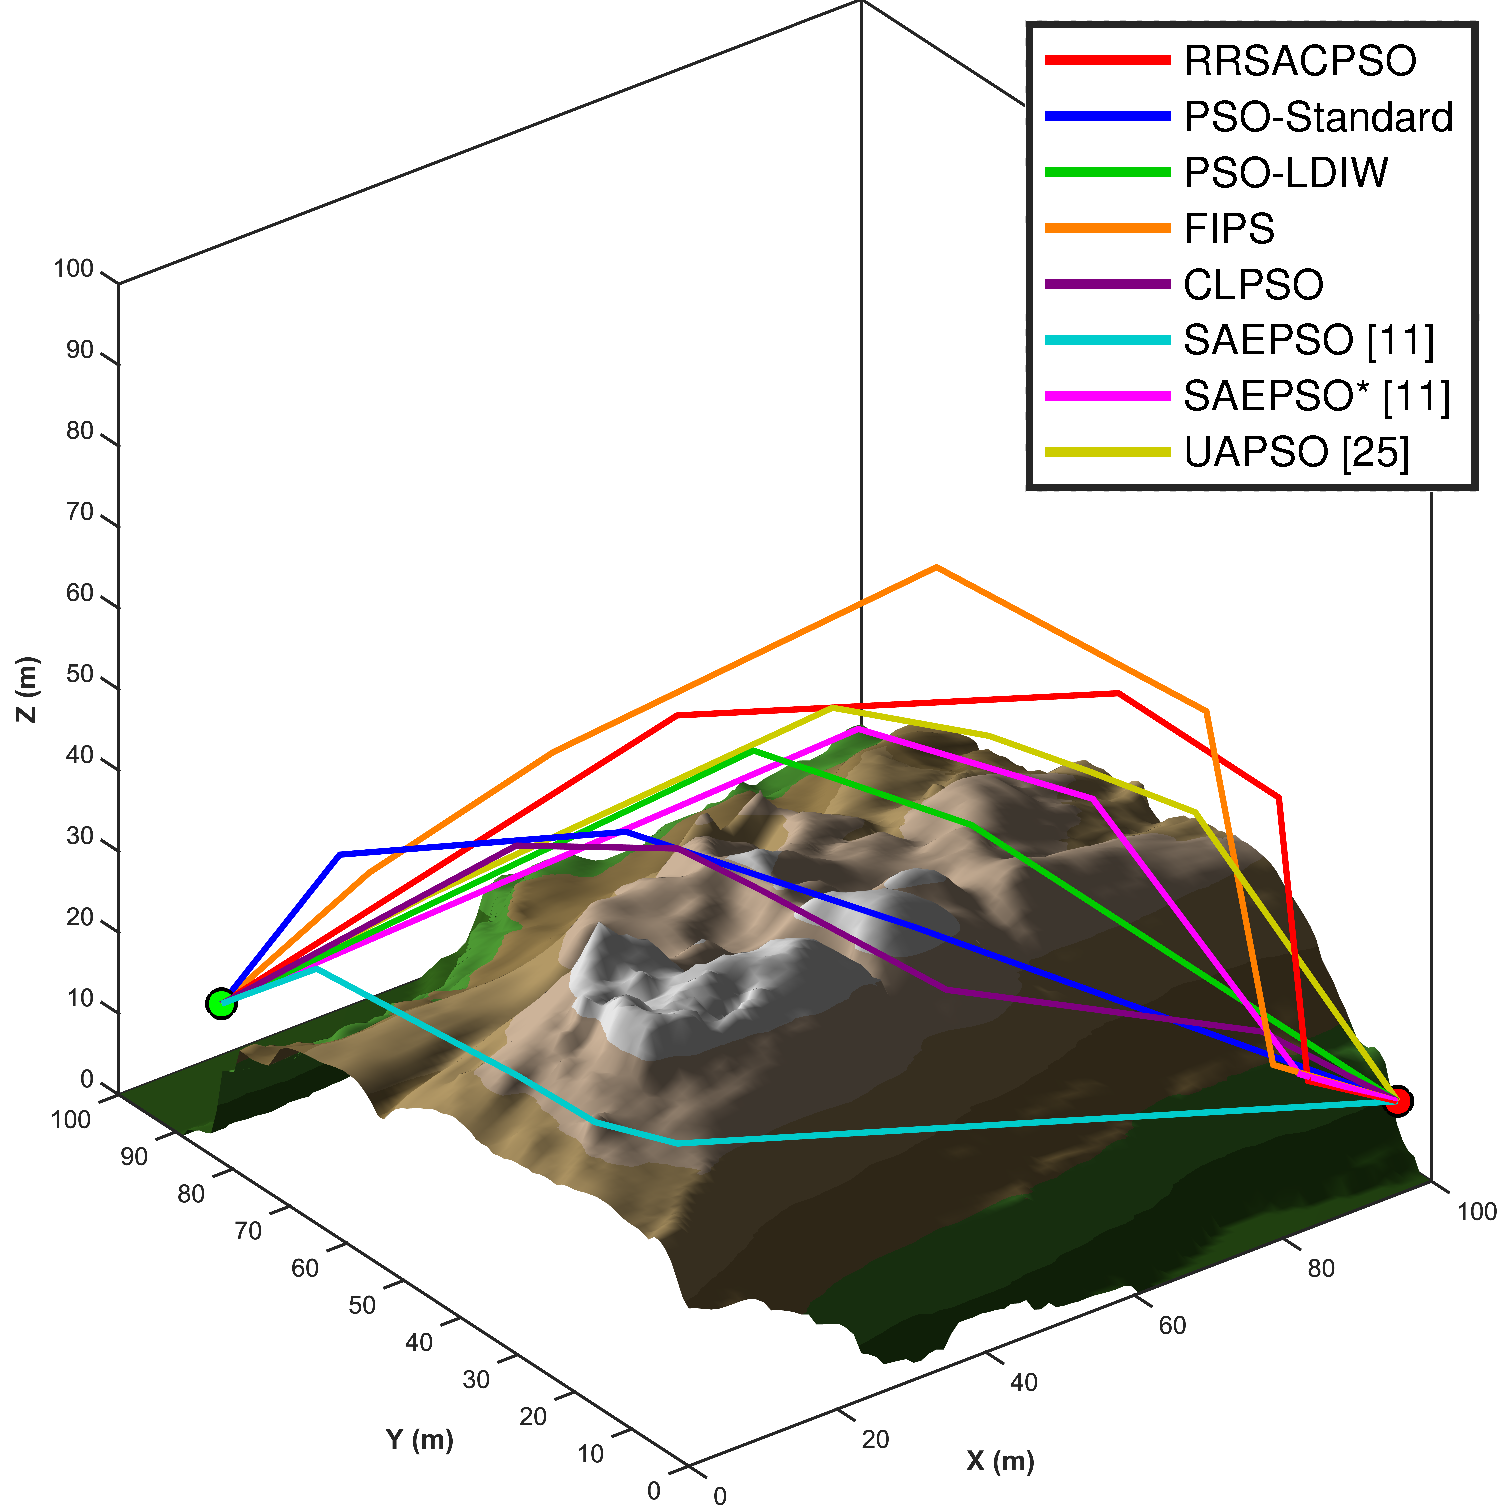
\includegraphics[width=\linewidth,height=0.16\textheight,keepaspectratio]{data/others3chrismast/Scenario1_3D.pdf}
\caption{Scenario 1}
\end{subfigure}
\hfill
\begin{subfigure}{0.24\textwidth}
\centering
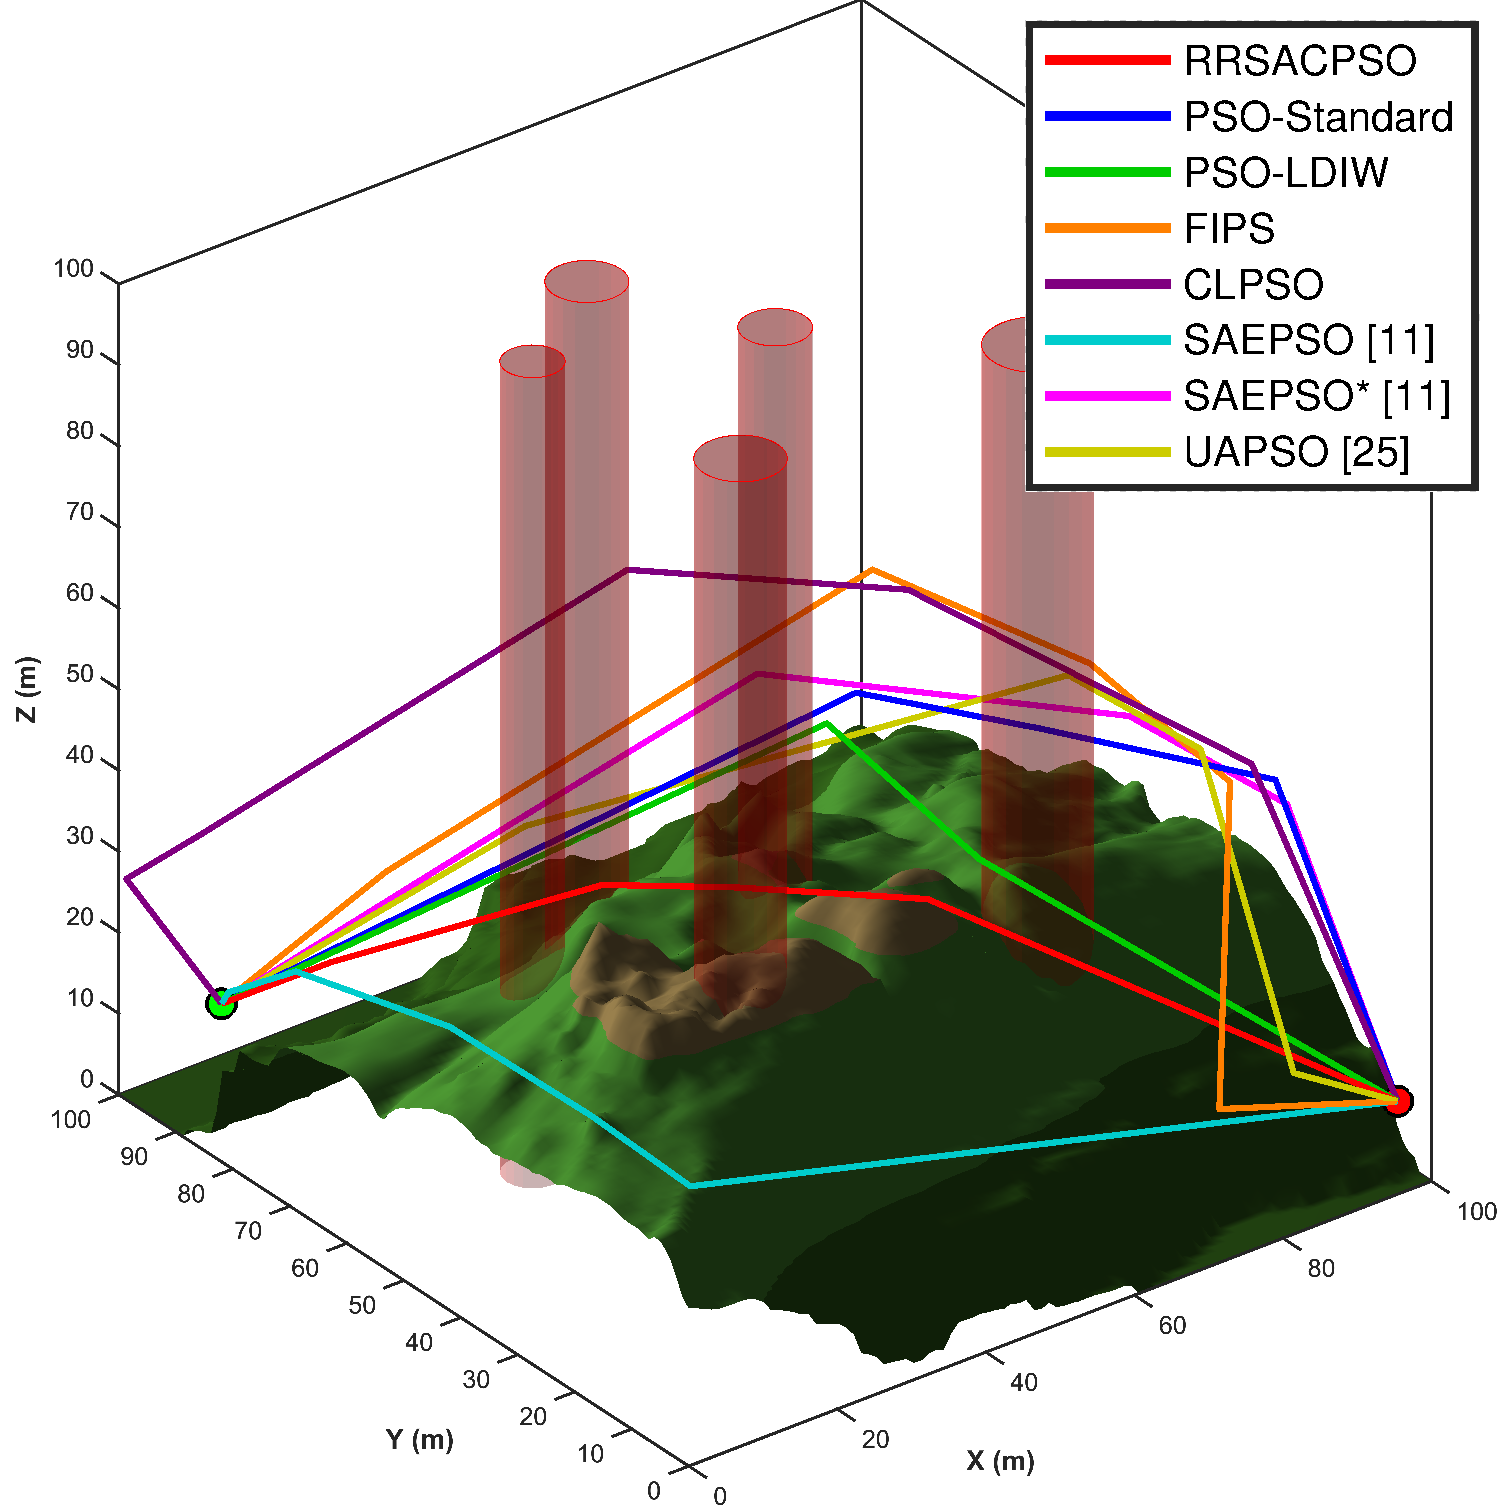
\includegraphics[width=\linewidth,height=0.16\textheight,keepaspectratio]{data/others3chrismast/Scenario2_3D.pdf}
\caption{Scenario 2}
\end{subfigure}
\hfill
\begin{subfigure}{0.24\textwidth}
\centering
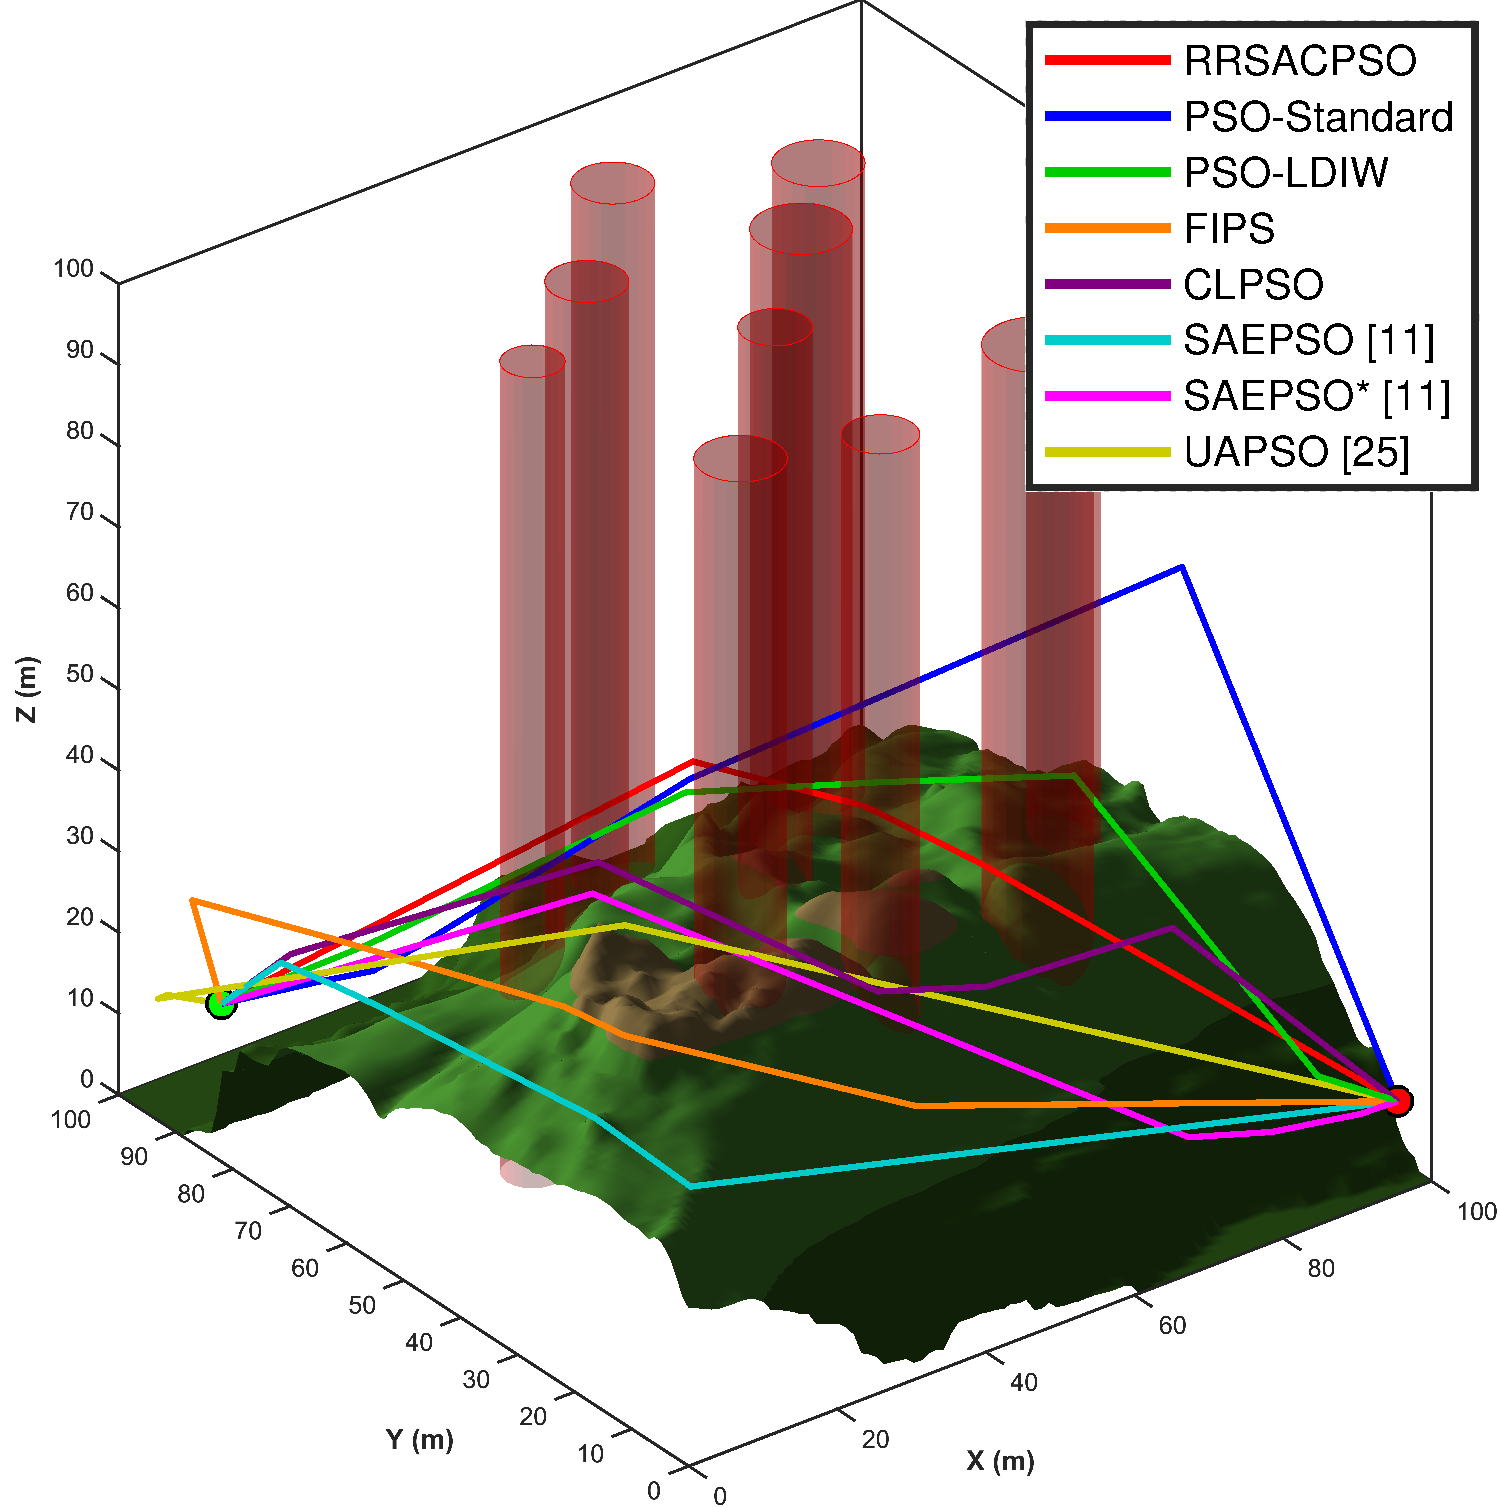
\includegraphics[width=\linewidth,height=0.16\textheight,keepaspectratio]{data/others3chrismast/Scenario3_3D.pdf}
\caption{Scenario 3}
\end{subfigure}
\hfill
\begin{subfigure}{0.24\textwidth}
\centering
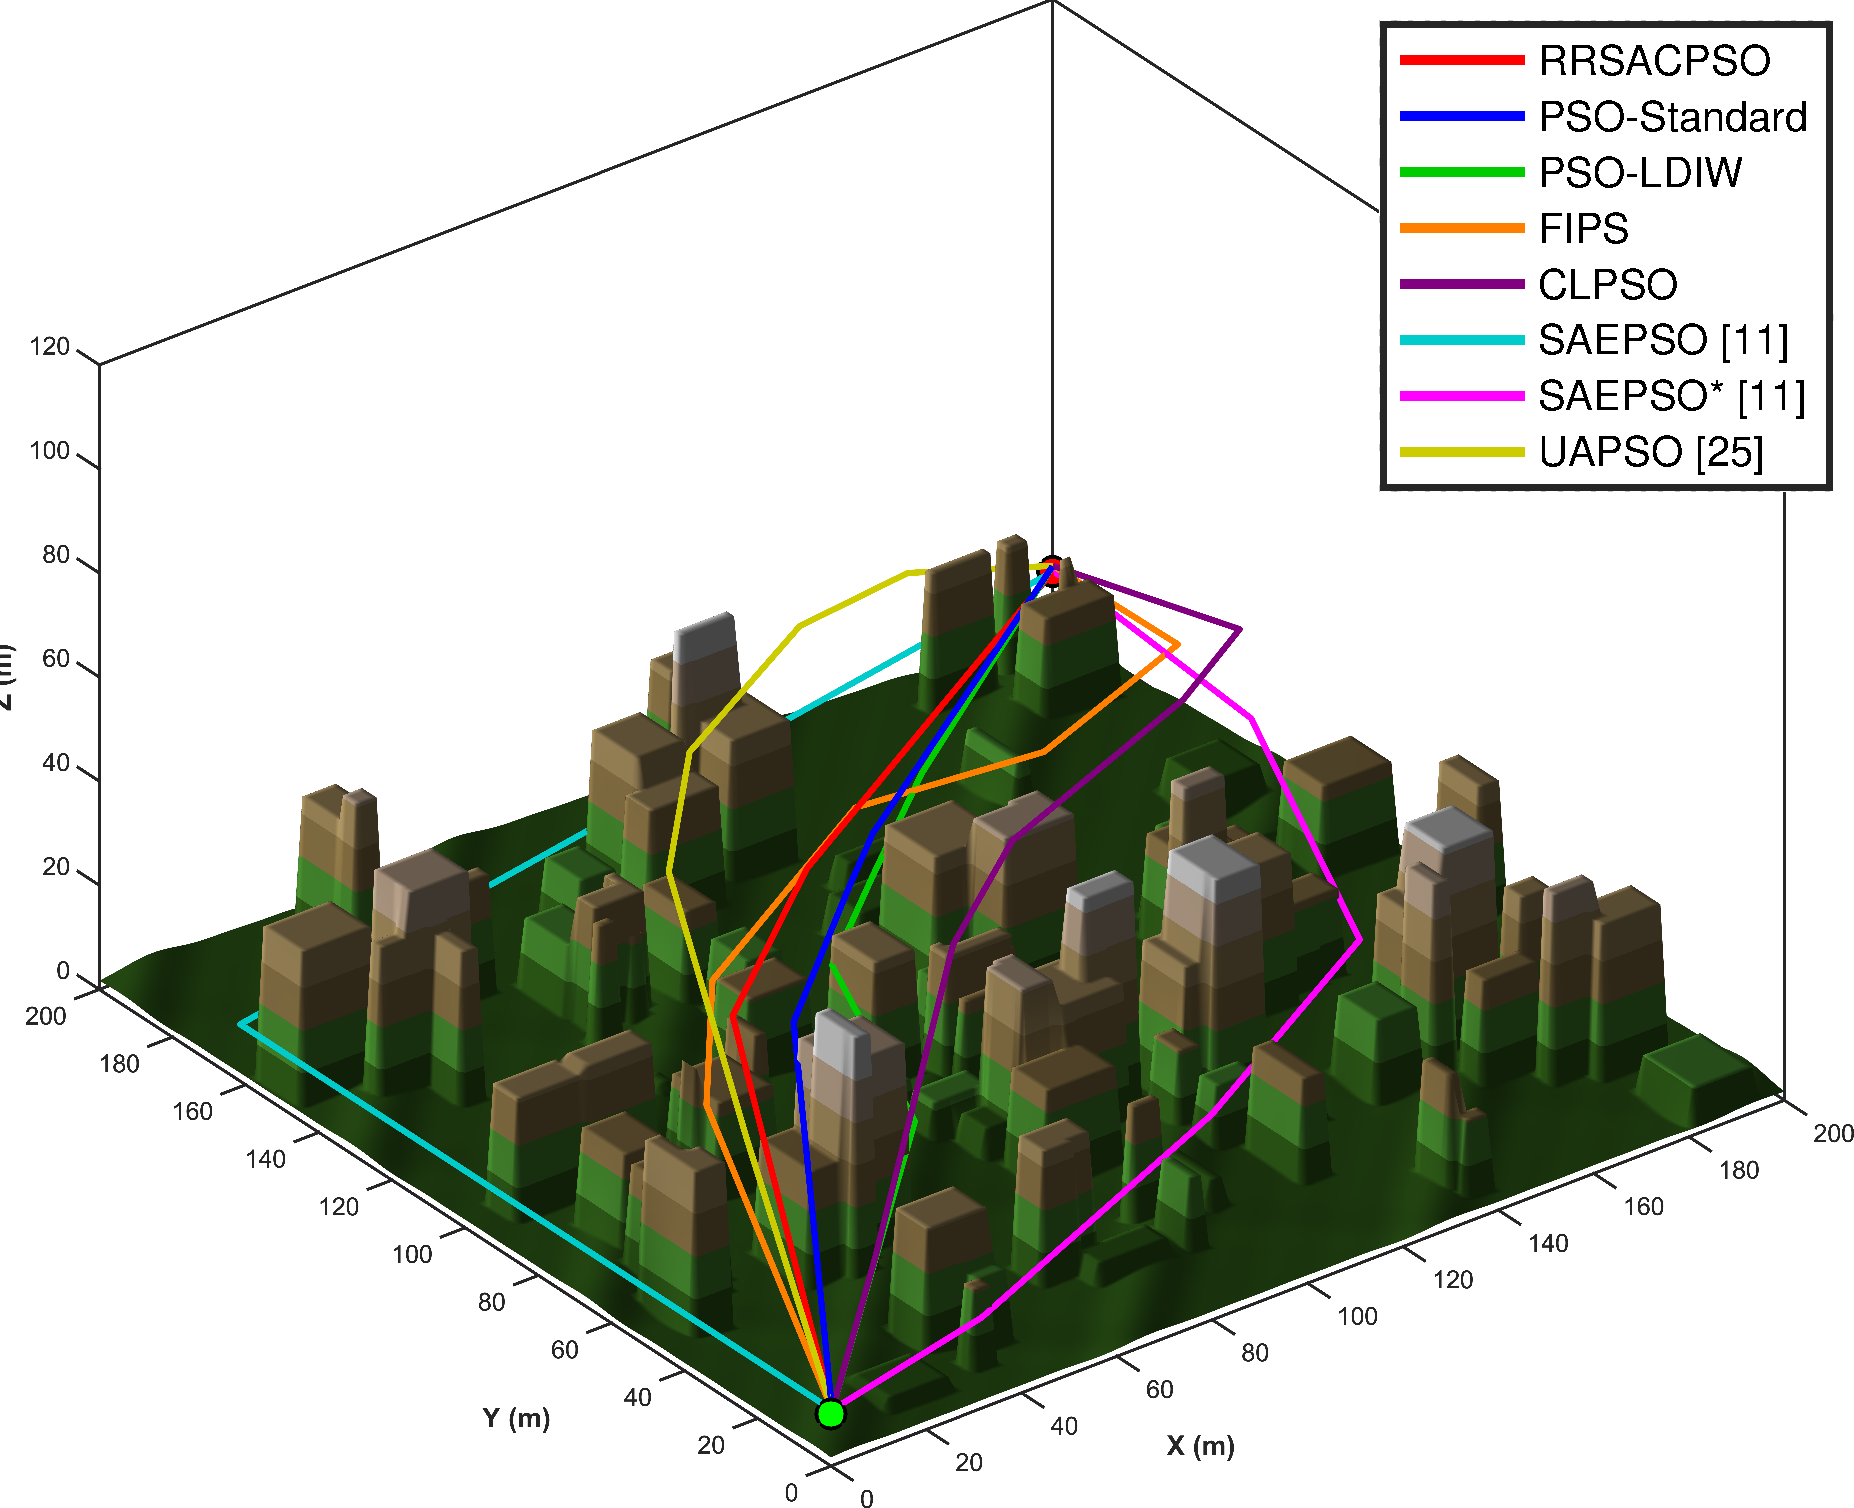
\includegraphics[width=\linewidth,height=0.16\textheight,keepaspectratio]{data/others3chrismast/Scenario4_3D.pdf}
\caption{Scenario 4}
\end{subfigure}
\caption{Classical/adaptive-PSO 3D trajectory comparisons across the four benchmark scenarios.}
\label{fig:others_3d_grid}
\end{figure*}

\begin{figure*}[!t]
\centering
\begin{subfigure}{0.24\textwidth}
\centering
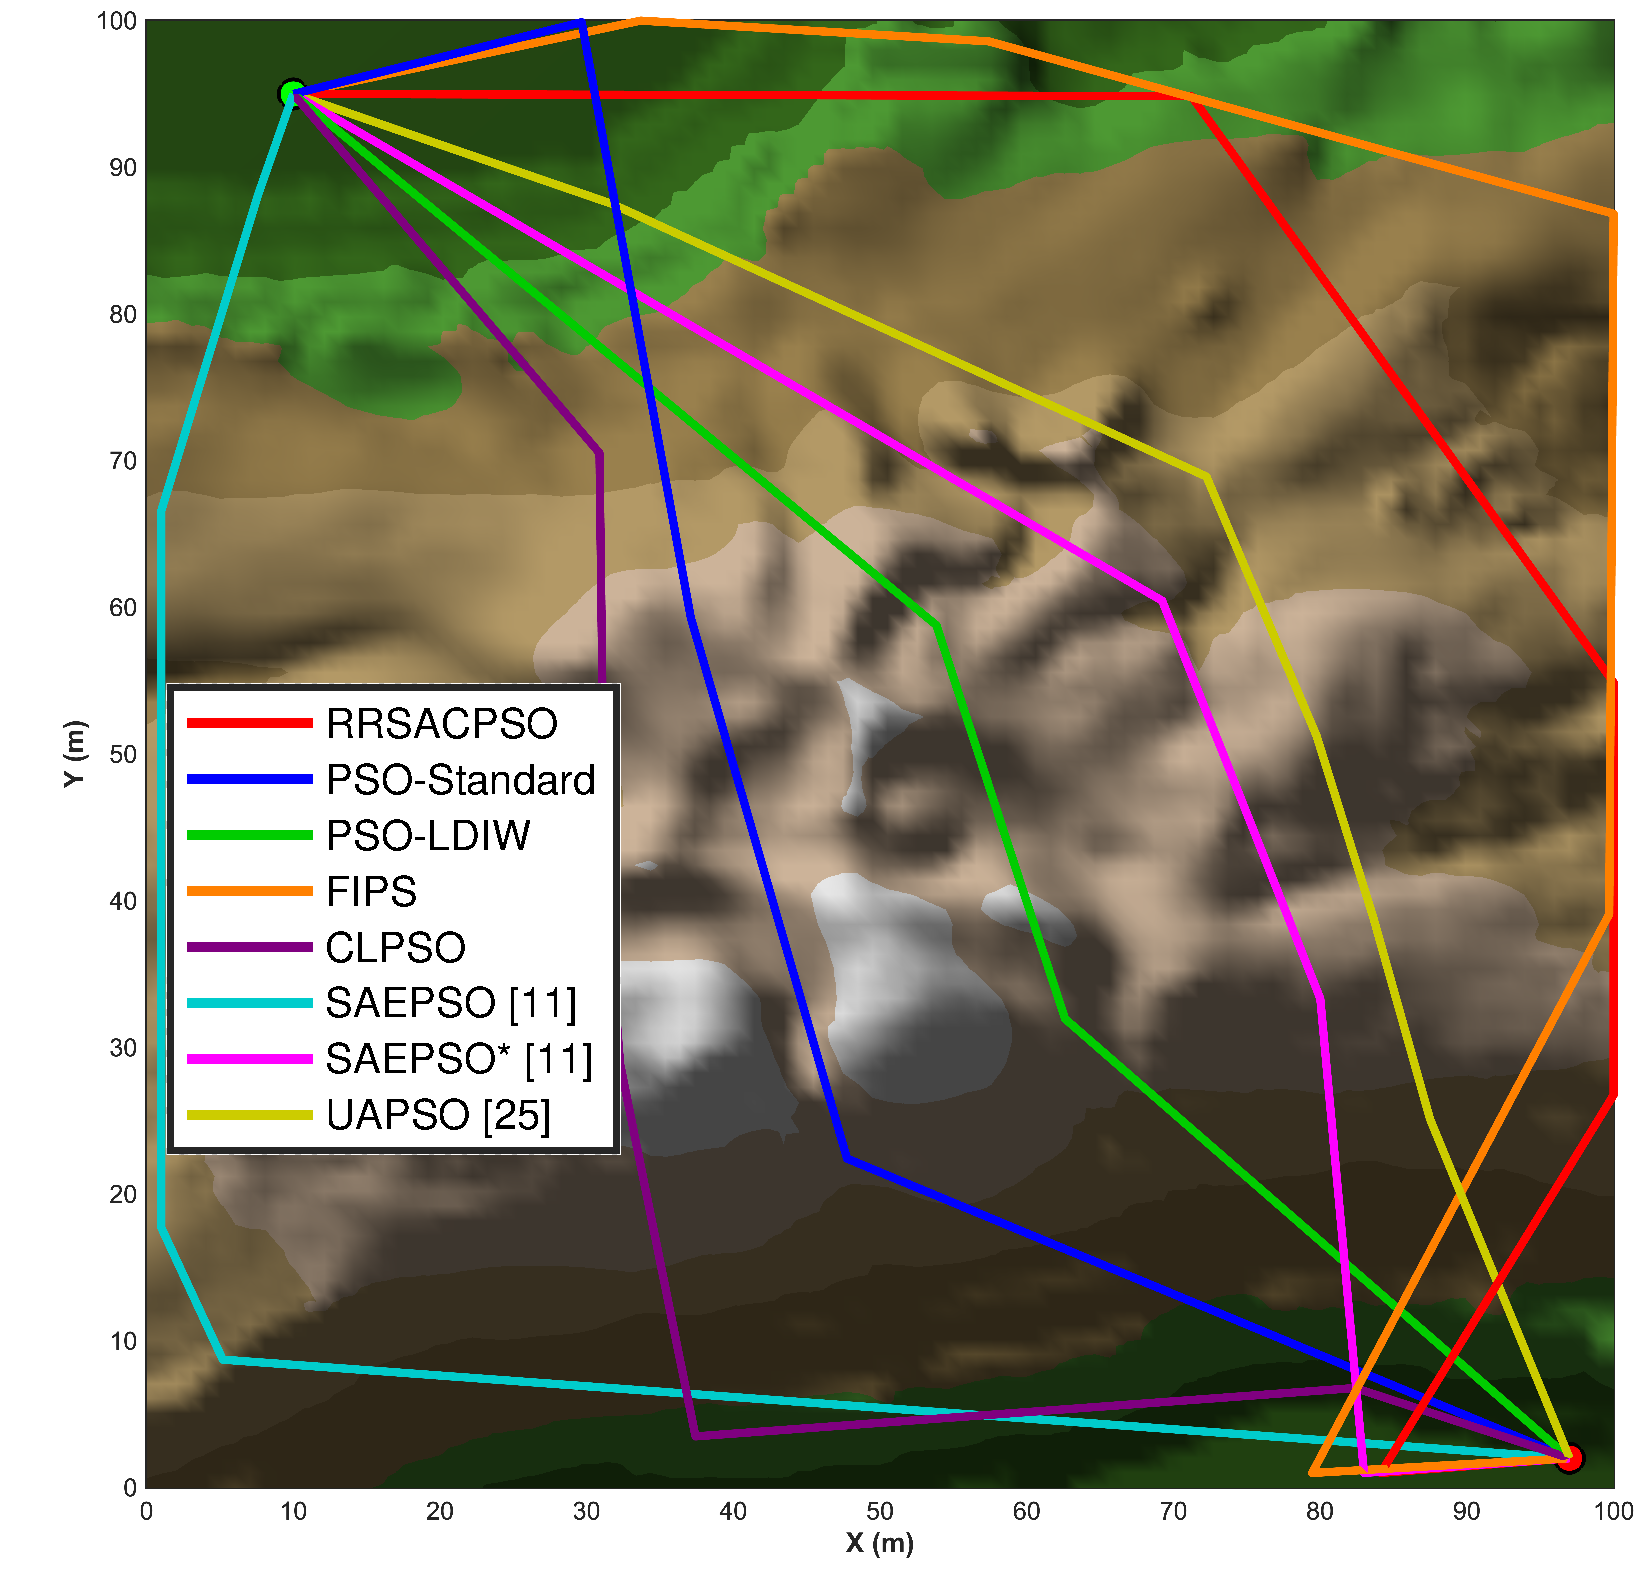
\includegraphics[width=\linewidth,height=0.16\textheight,keepaspectratio]{data/others3chrismast/Scenario1_TopView.pdf}
\caption{Scenario 1}
\end{subfigure}
\hfill
\begin{subfigure}{0.24\textwidth}
\centering
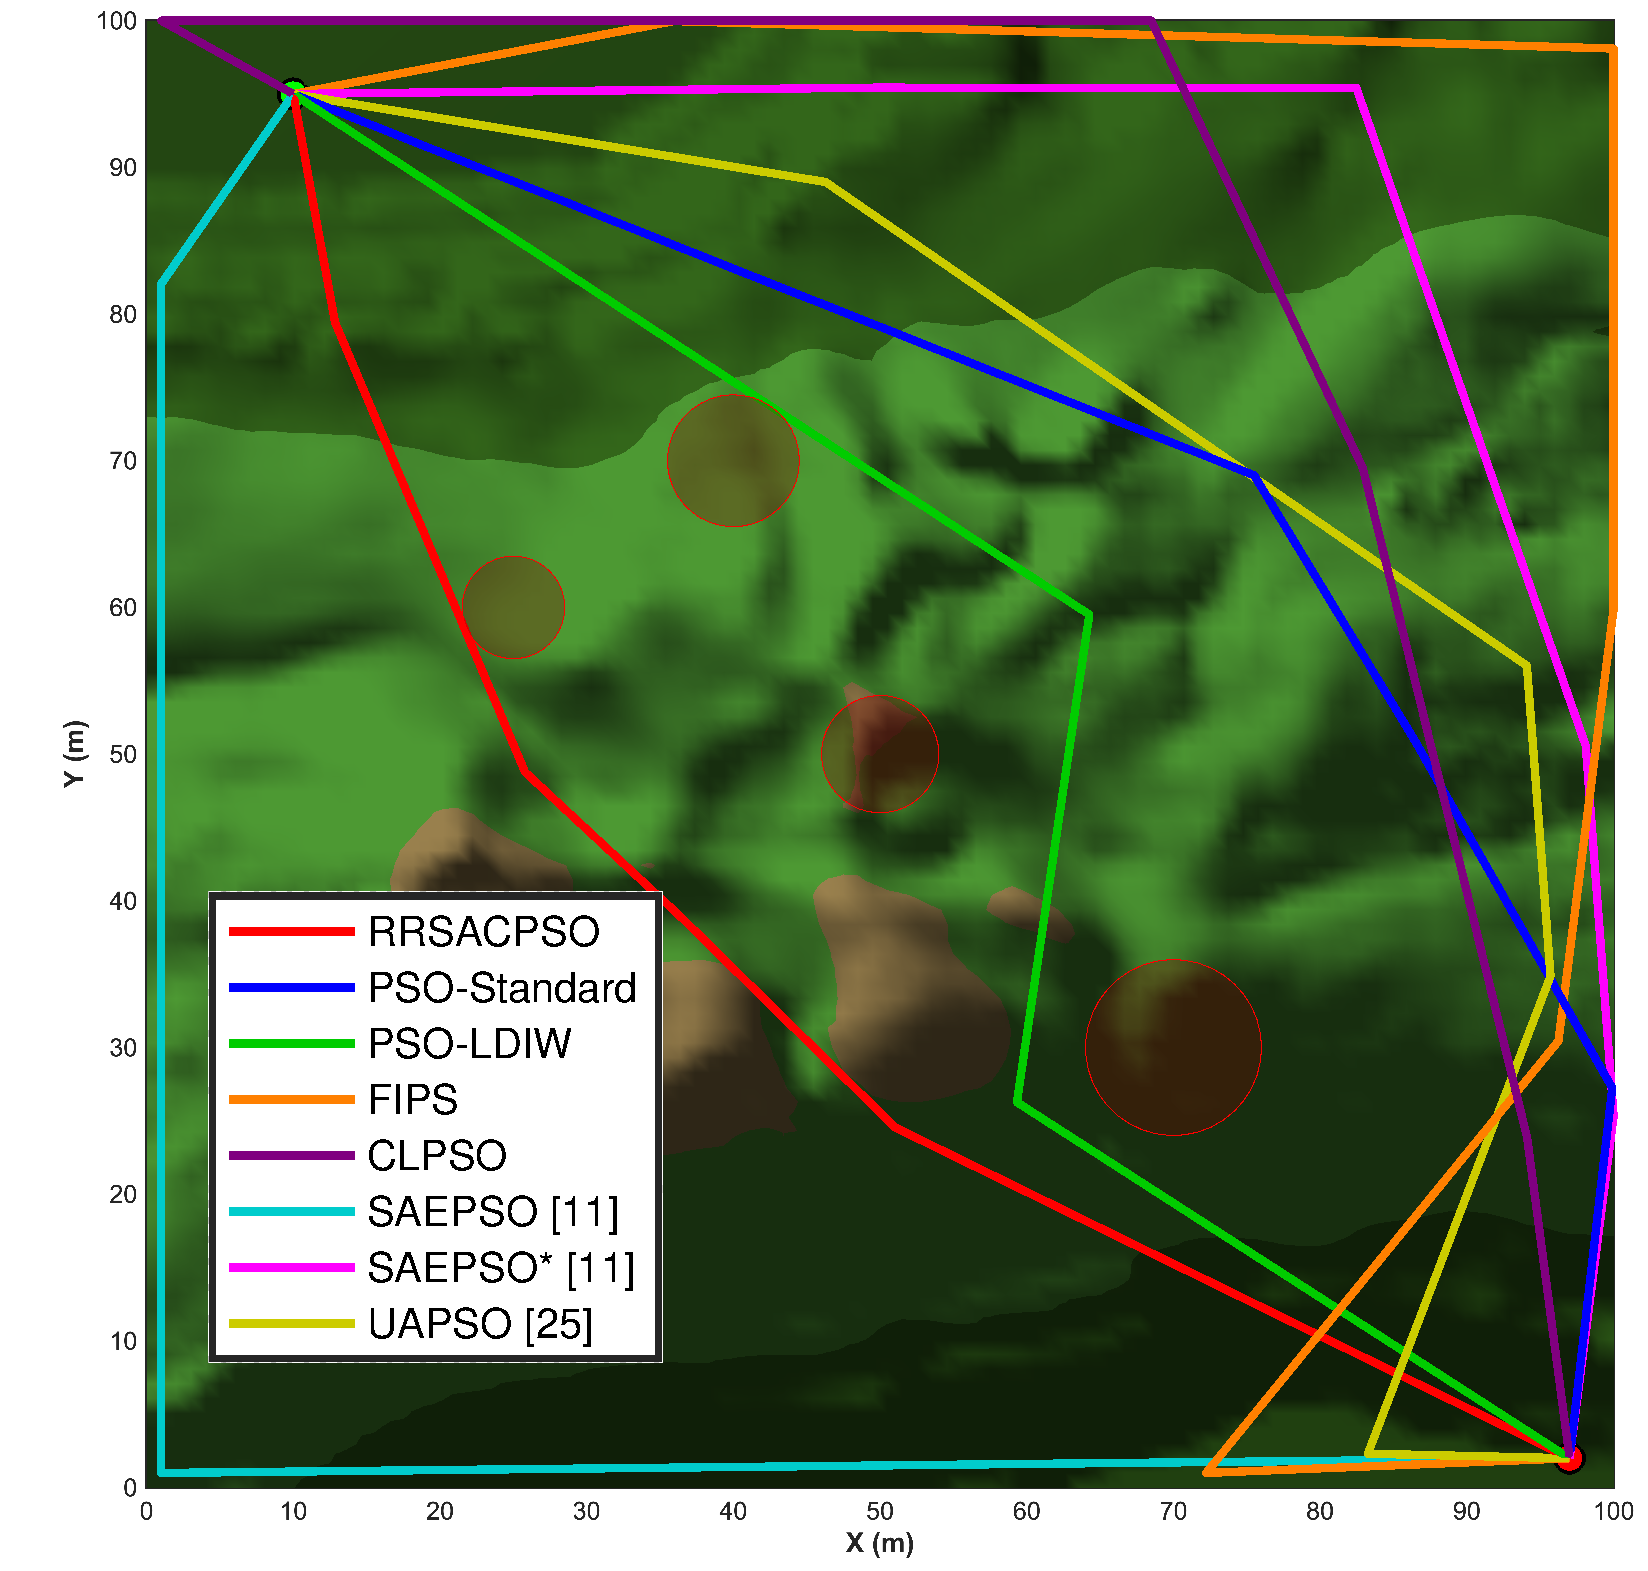
\includegraphics[width=\linewidth,height=0.16\textheight,keepaspectratio]{data/others3chrismast/Scenario2_TopView.pdf}
\caption{Scenario 2}
\end{subfigure}
\hfill
\begin{subfigure}{0.24\textwidth}
\centering
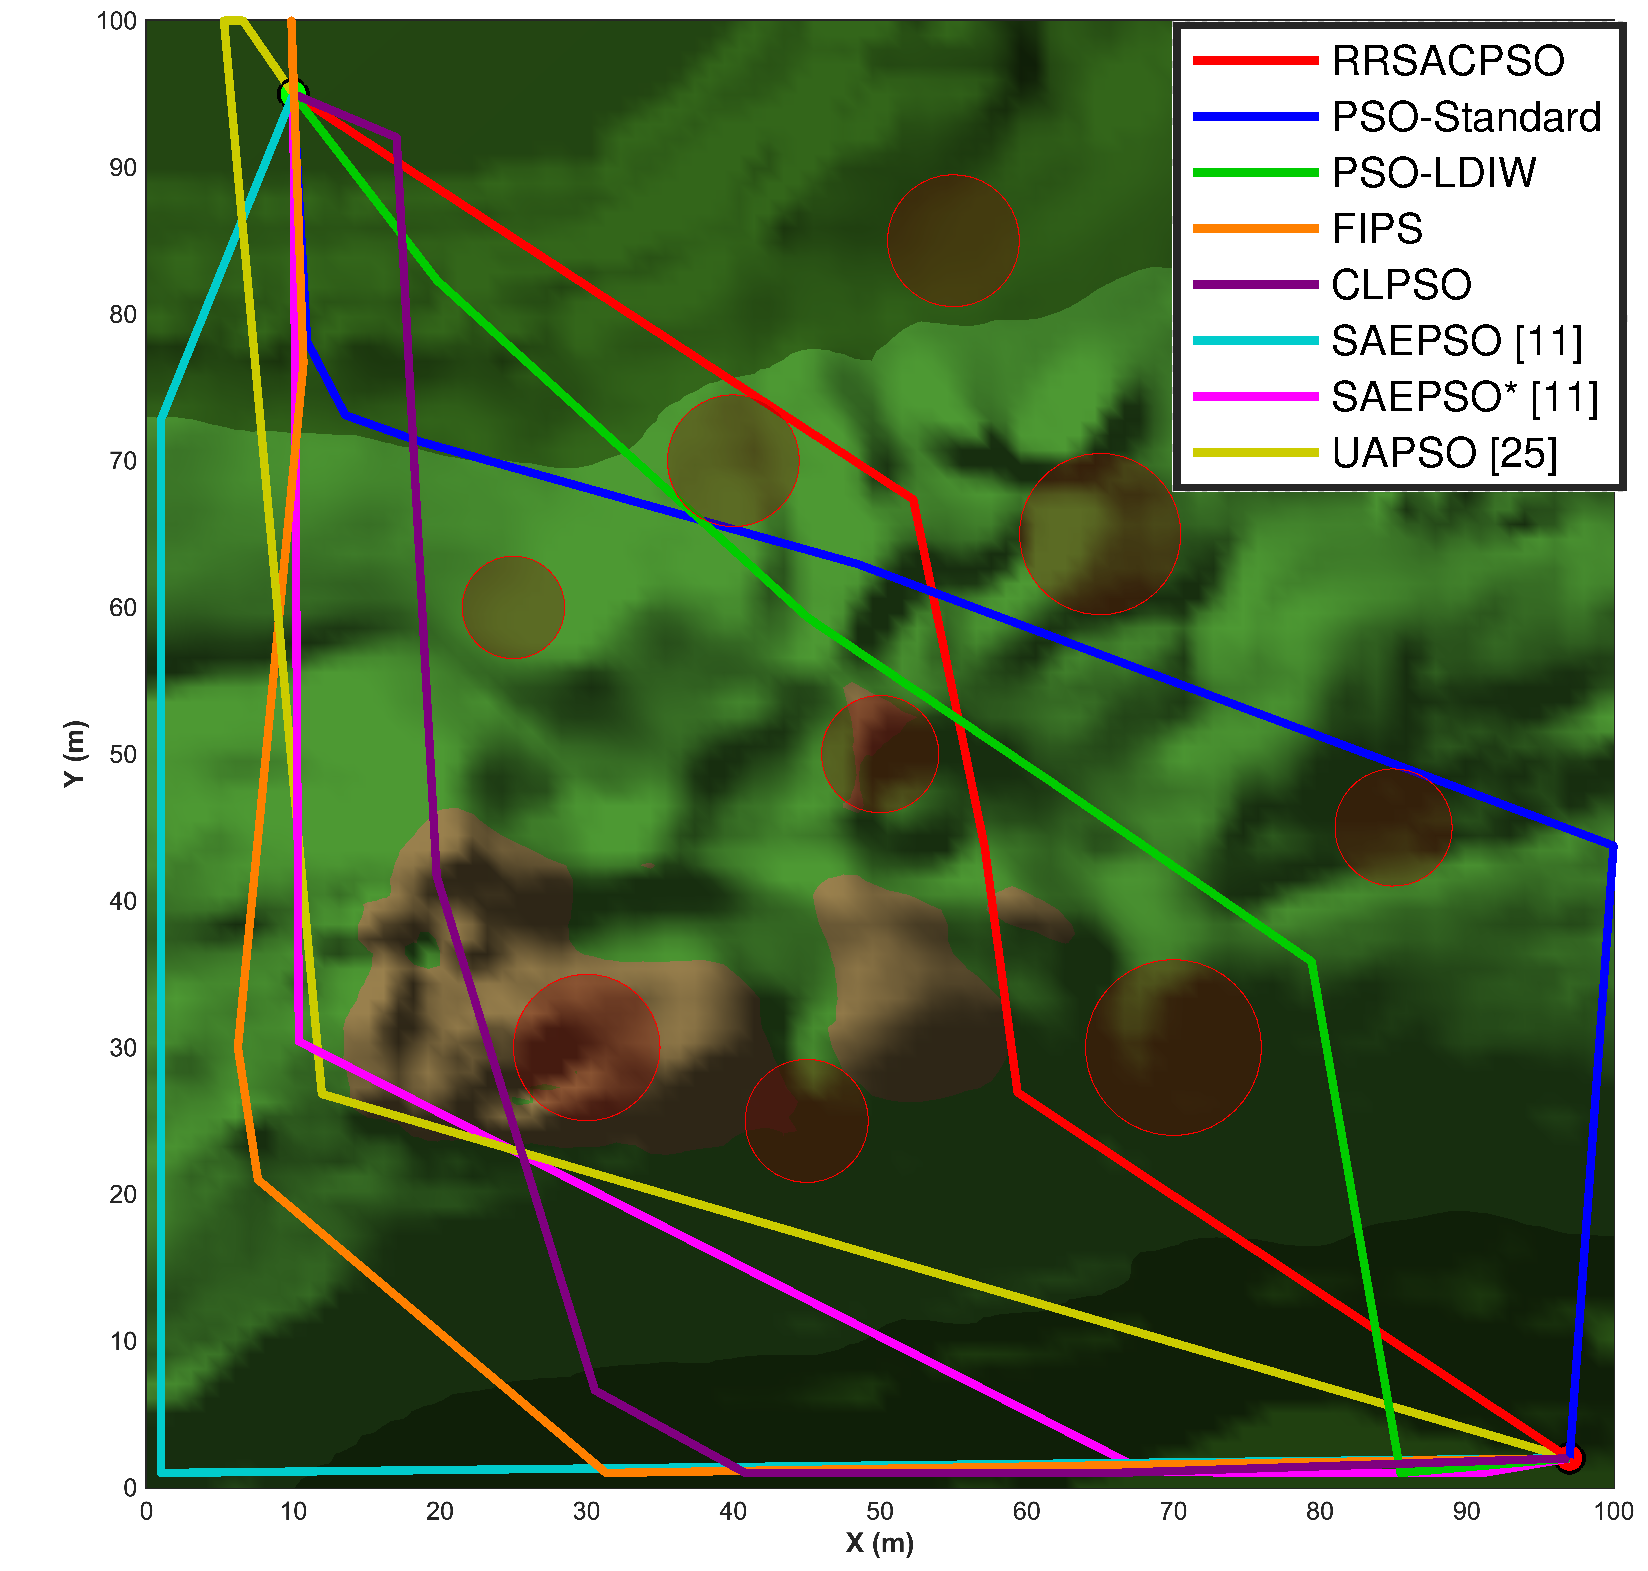
\includegraphics[width=\linewidth,height=0.16\textheight,keepaspectratio]{data/others3chrismast/Scenario3_TopView.pdf}
\caption{Scenario 3}
\end{subfigure}
\hfill
\begin{subfigure}{0.24\textwidth}
\centering
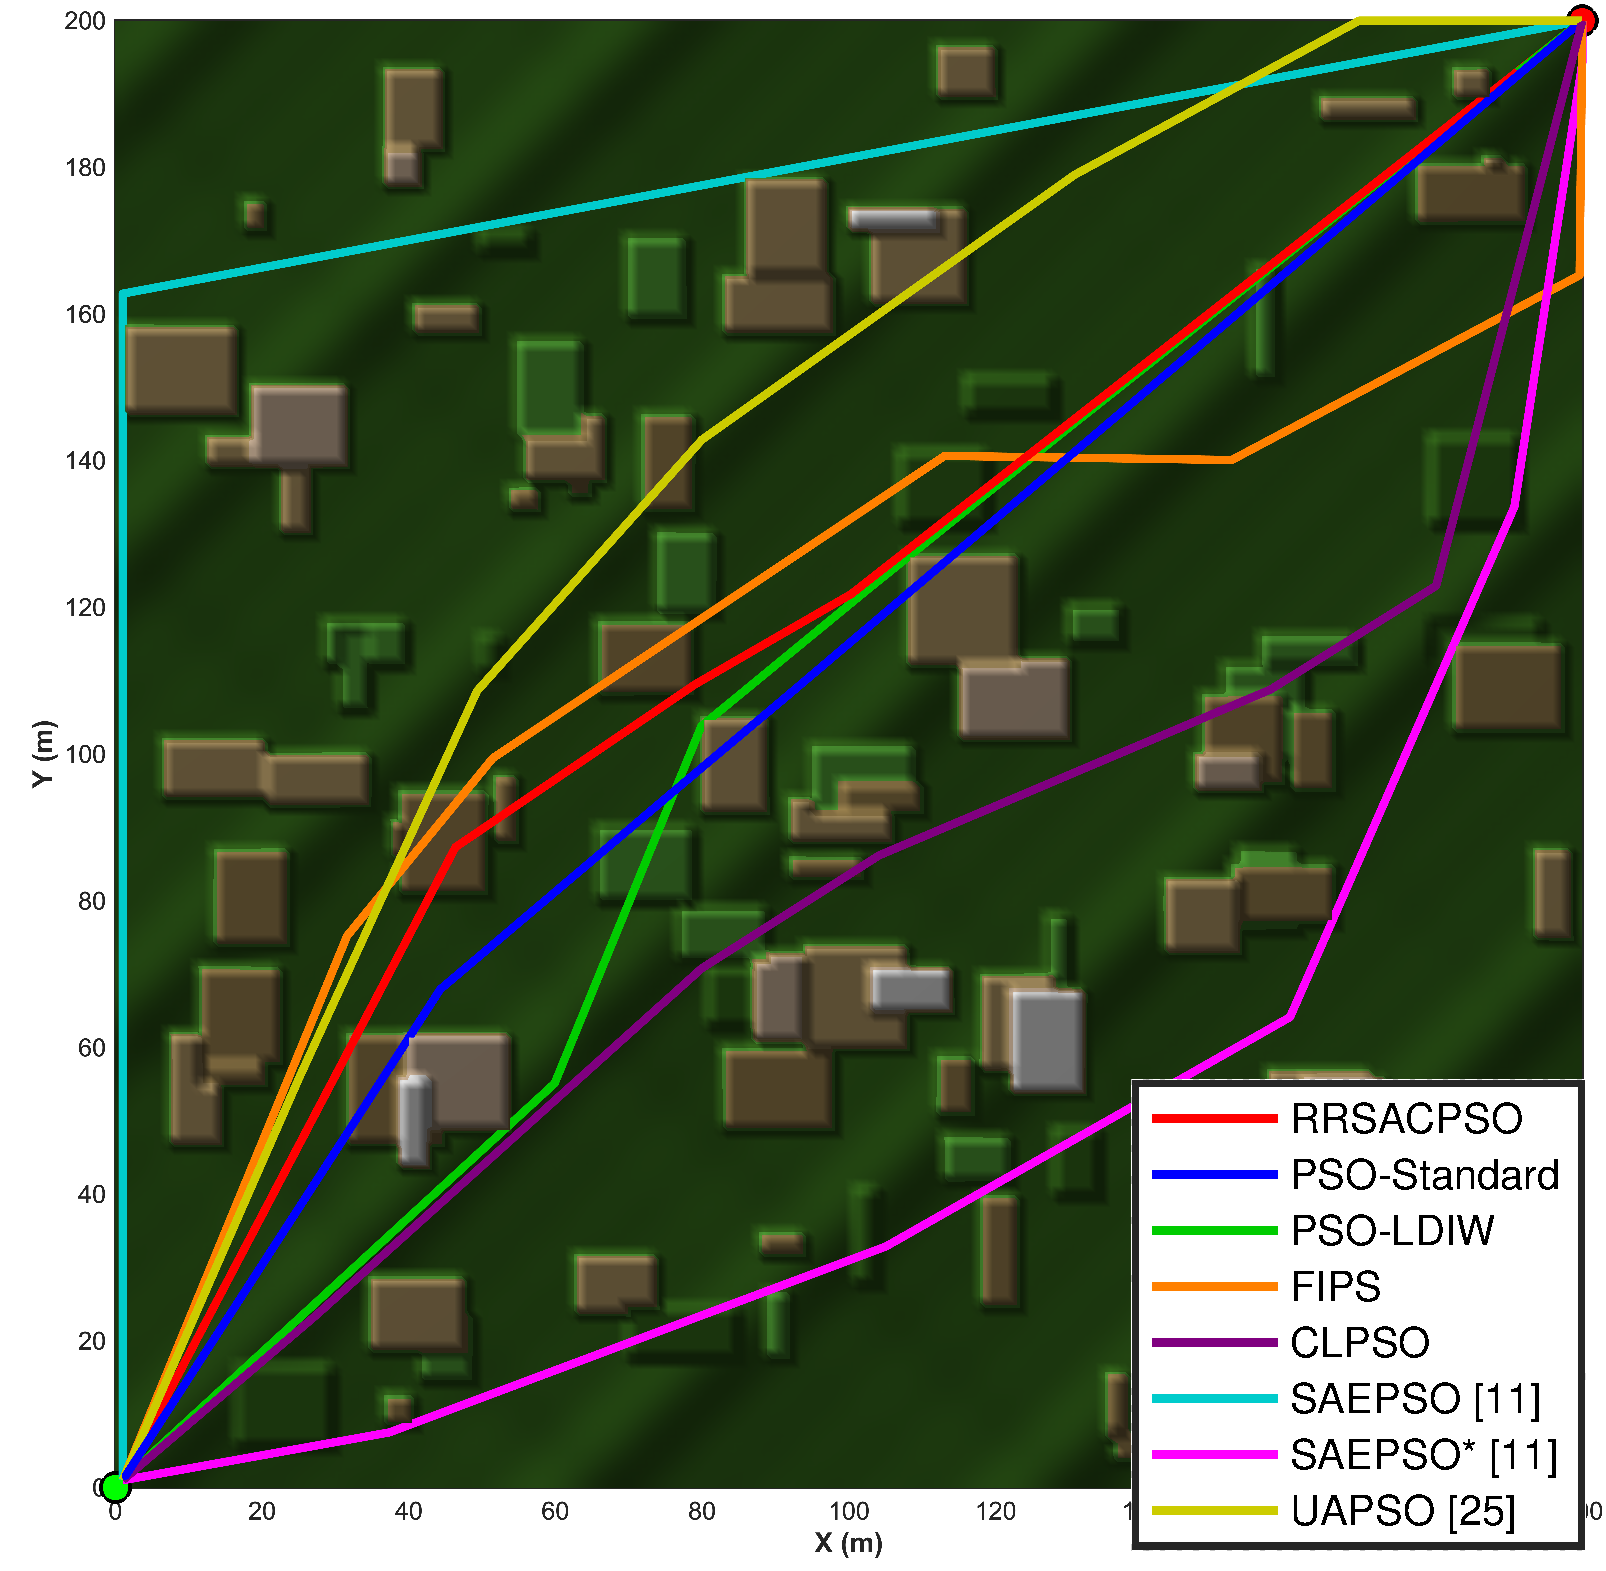
\includegraphics[width=\linewidth,height=0.16\textheight,keepaspectratio]{data/others3chrismast/Scenario4_TopView.pdf}
\caption{Scenario 4}
\end{subfigure}
\caption{Classical/adaptive-PSO top-view trajectory comparisons across the four benchmark scenarios.}
\label{fig:others_topview_grid}
\end{figure*}

\begin{figure*}[!t]
\centering
\begin{subfigure}{0.48\textwidth}
\centering
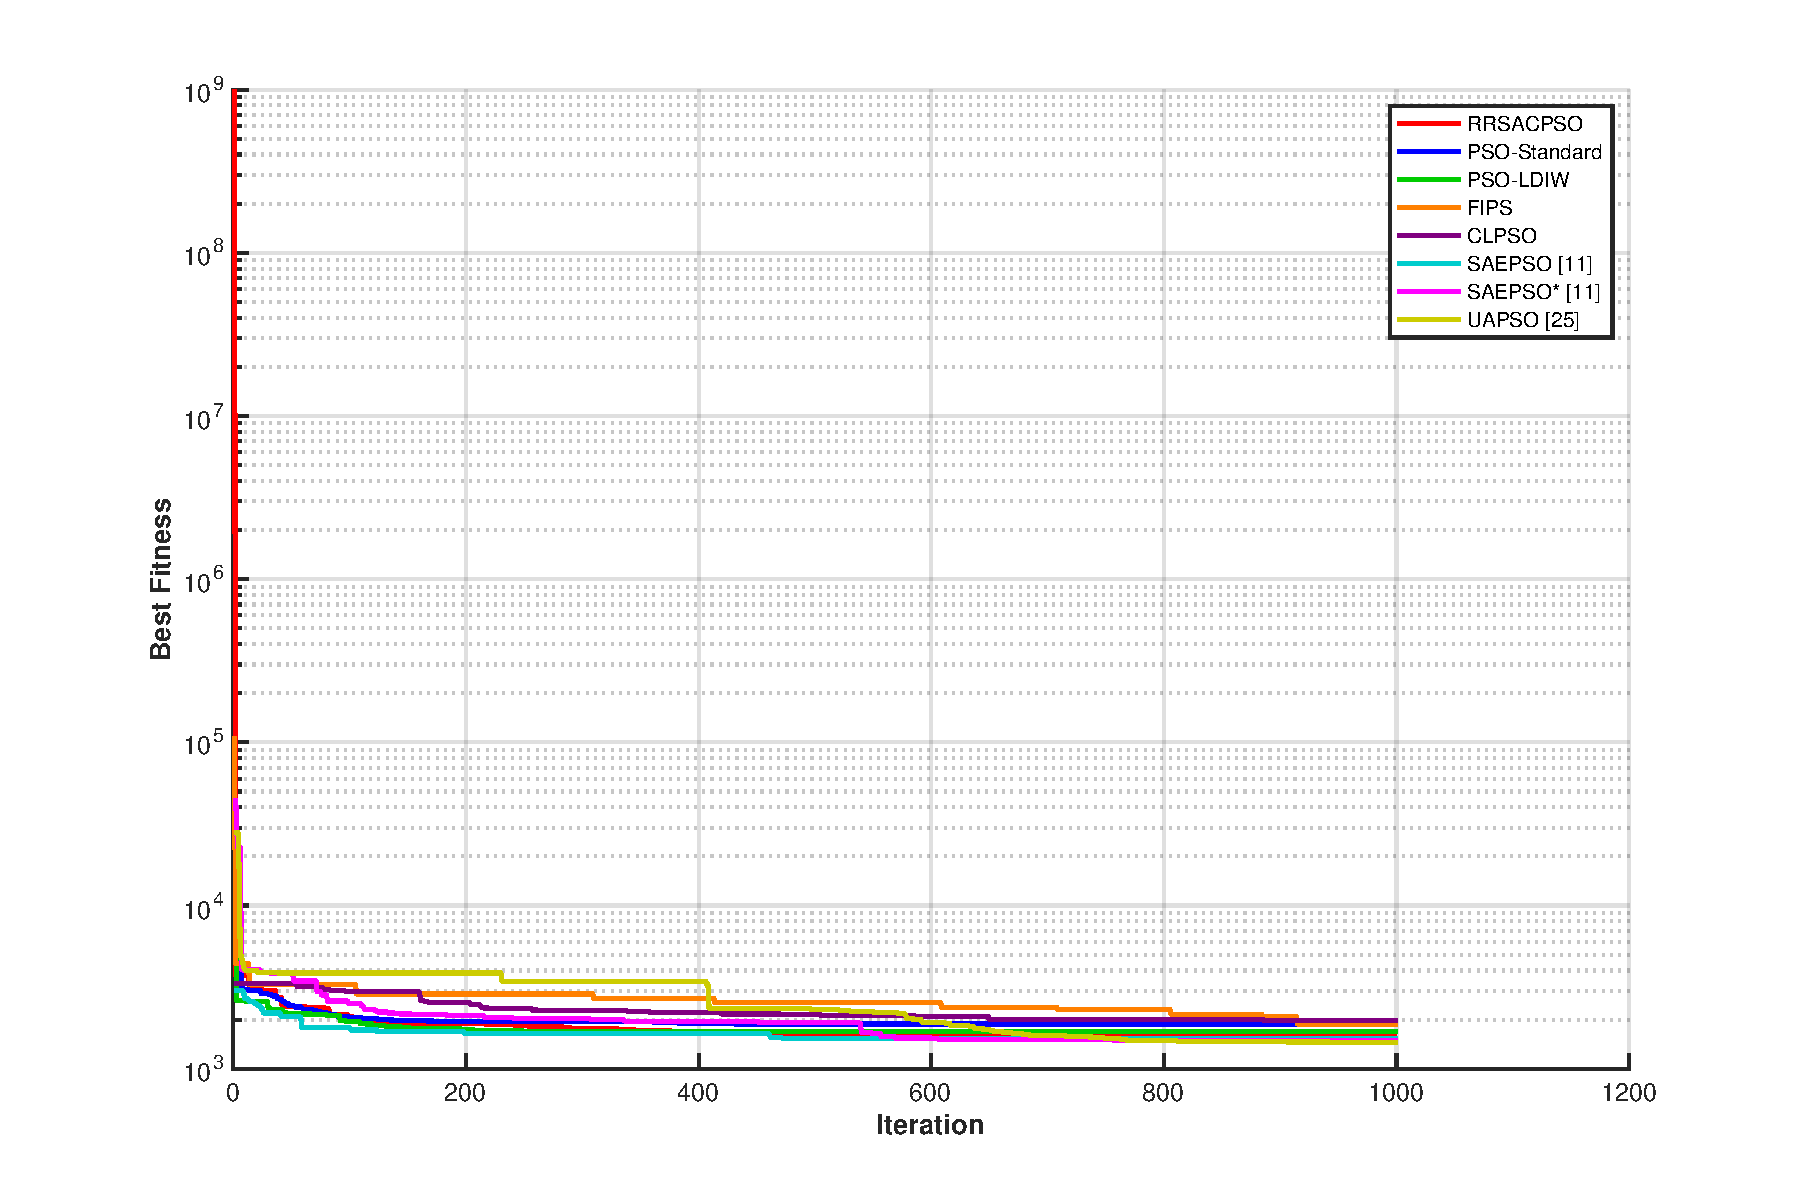
\includegraphics[width=\linewidth,height=0.18\textheight,keepaspectratio]{data/others3chrismast/Convergence_Comparison.pdf}
\caption{Convergence}
\end{subfigure}
\hfill
\begin{subfigure}{0.48\textwidth}
\centering
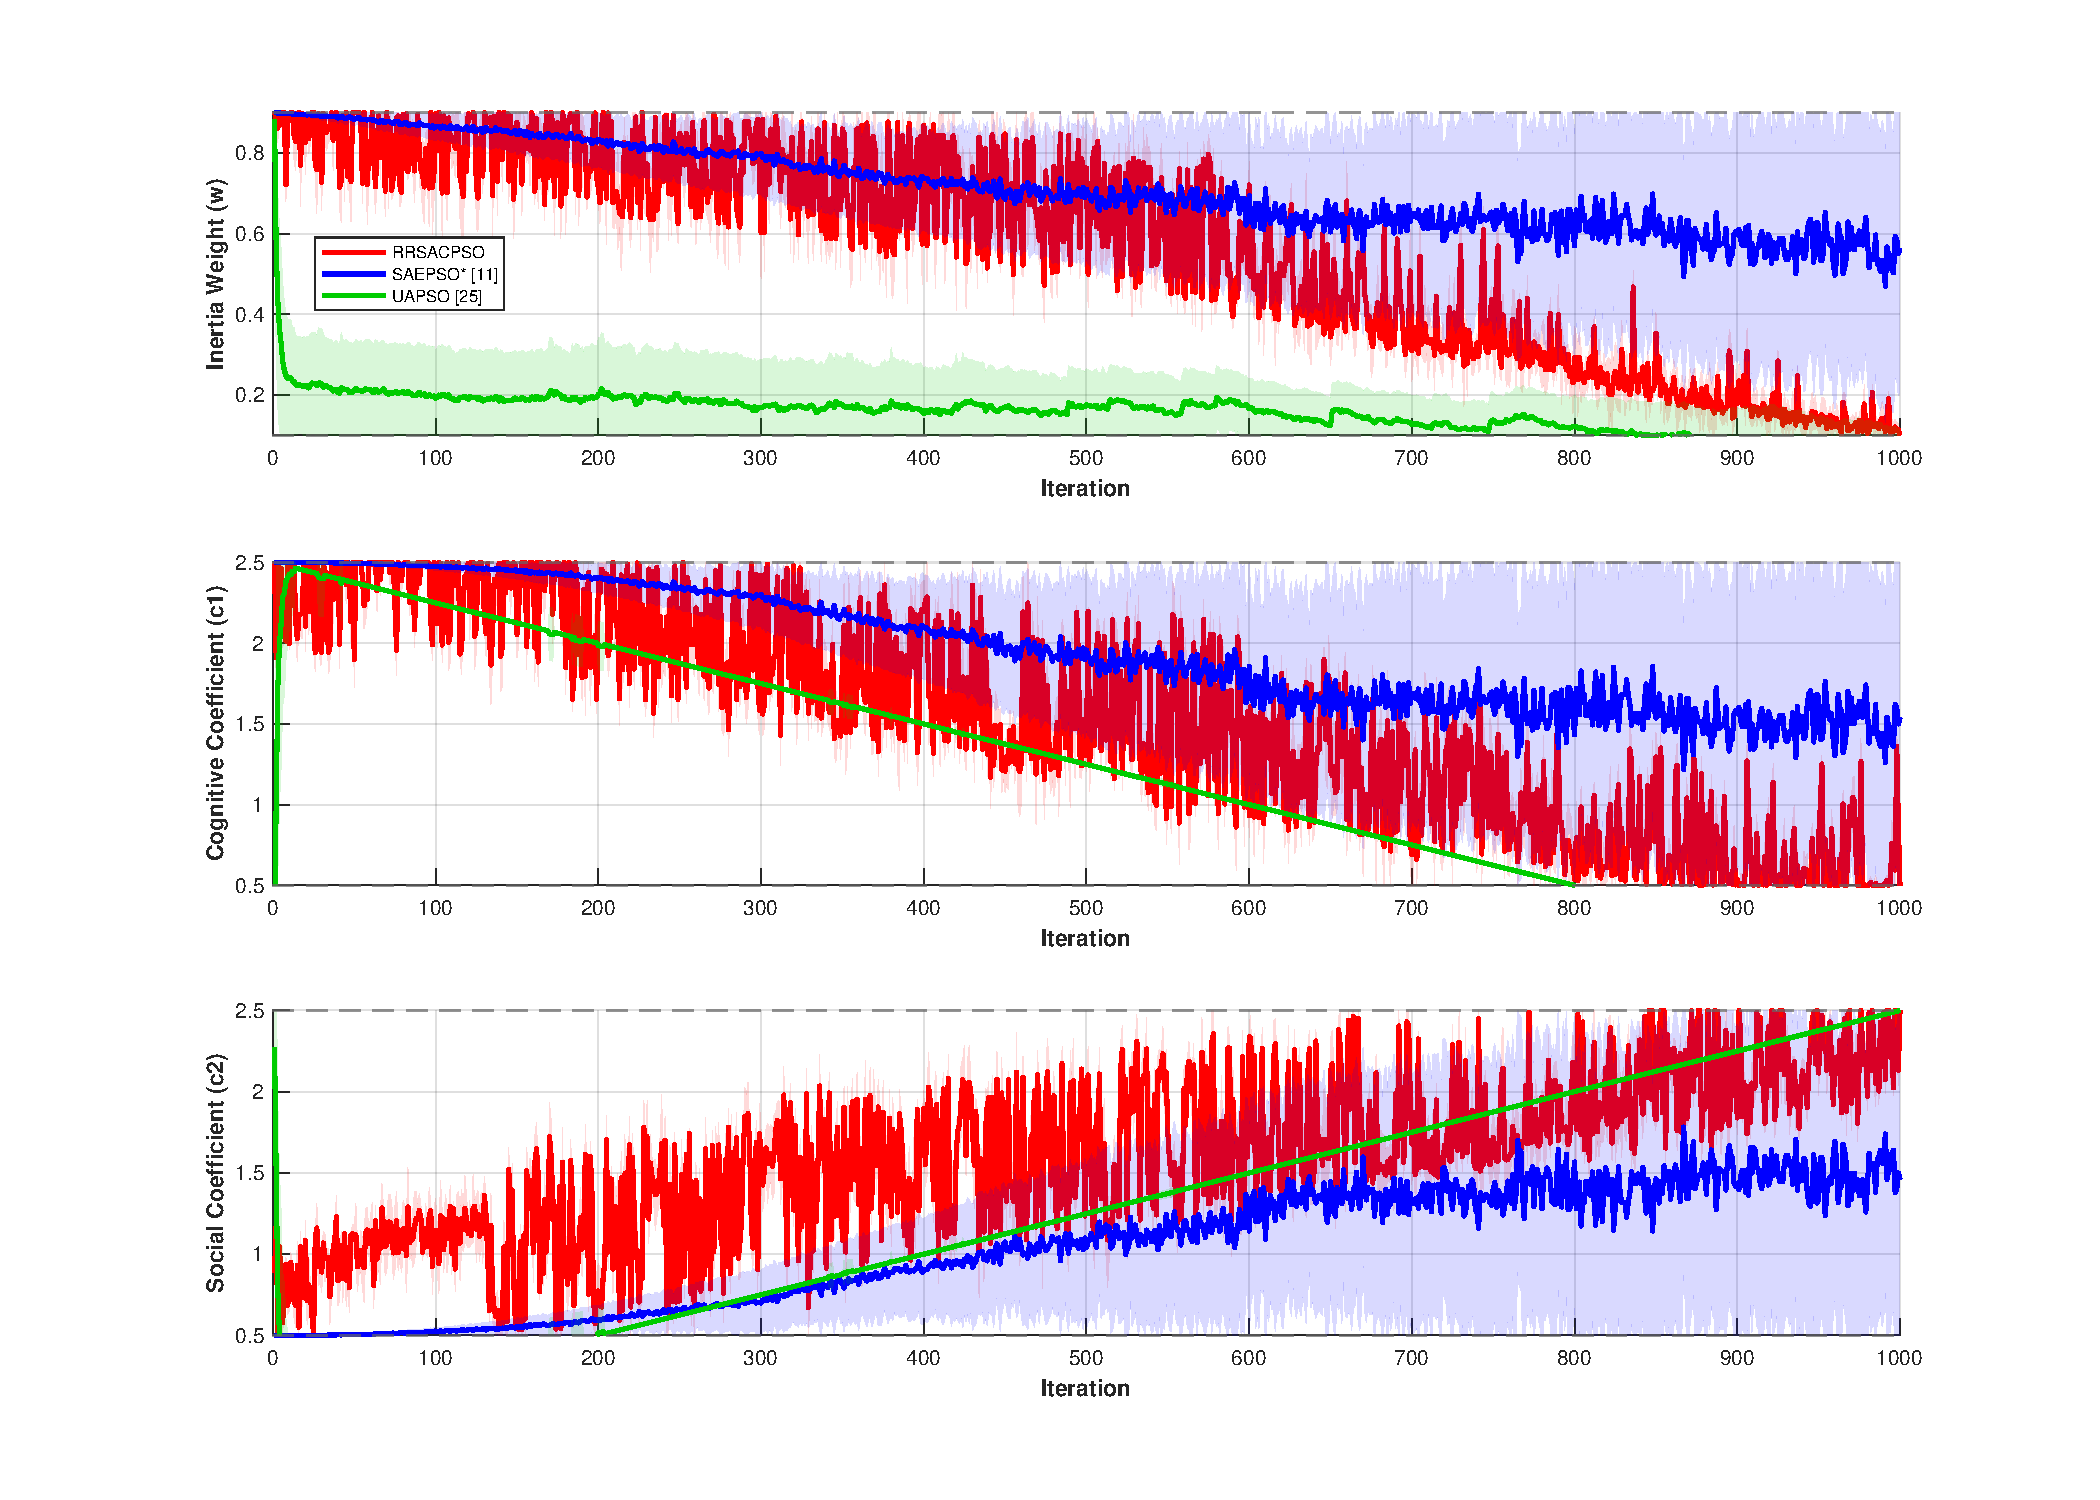
\includegraphics[width=\linewidth,height=0.18\textheight,keepaspectratio]{data/others3chrismast/Parameter_Tracking.pdf}
\caption{Parameter tracking}
\end{subfigure}
\caption{Classical/adaptive-PSO convergence and parameter-tracking diagnostics.}
\label{fig:others_convergence_tracking}
\end{figure*}
\subsection{SAC Control Granularity and Attractor-Field Ablation}
\label{subsec:sac_granularity_ablation_results}
To probe the role of the control interface, we ran an internal four-mode ablation under the same retained SAC backbone used throughout this paper.
All four modes use the same 15D temporal-summary state, relative fitness-improvement reward, twin-critic target-network training, and paired-seed protocol, with only the action-to-parameter mapping changed.
Within this subsection, `SACPSO-Global', `SACPSO-5Subgroup', and `SACPSO-PerParticle' are matched internal baselines and should not be confused with the external SAC-SAPSO method in Table~\ref{tab:rl_comparison}.
`SACPSO-Global' applies one coefficient triplet to the full swarm, `SACPSO-5Subgroup' assigns one triplet per fixed subgroup, and `SACPSO-PerParticle' outputs direct particle-wise coefficients.
AFSACPSO retains the same plain SAC controller but expands a compact 9D latent action into particle-wise coefficients through attractor-field modulation with geometric context signals, whereas the three internal baselines map their actions directly to coefficient values.
For the current 100-particle benchmark, these modes correspond to 3D, 15D, 300D, and 9D latent-action control spaces, respectively.

Table~\ref{tab:sac_granularity_ablation} shows that the pretrained same-backbone ablation should be read as a control-interface comparison rather than as a blanket ranking of the proposed method.
SACPSO-Global attains the lowest mean fitness in all four scenarios, but AFSACPSO remains competitive because none of those advantages are significant after Holm correction.
At the same time, AFSACPSO is significantly better than SACPSO-5Subgroup in Scenario 1 and significantly better than SACPSO-PerParticle in Scenarios 1 and 2, while remaining statistically indistinguishable from both alternatives on the harder Scenarios 3 and 4.
\begin{table*}[!t]
\centering
\small
\resizebox{\textwidth}{!}{%
\begin{tabular}{lccc ccc ccc ccc}
\hline
\multirow{2}{*}{Algorithm} & \multicolumn{3}{c}{Scenario 1} & \multicolumn{3}{c}{Scenario 2} & \multicolumn{3}{c}{Scenario 3} & \multicolumn{3}{c}{Scenario 4} \\
\cline{2-13}
 & Fitness & Time & TTest & Fitness & Time & TTest & Fitness & Time & TTest & Fitness & Time & TTest \\
\hline
AFSACPSO & 1607.24 $\pm$ 86.79 & 38.72 & --- & 1571.01 $\pm$ 104.64 & 35.73 & --- & 1586.71 $\pm$ 144.62 & 34.95 & --- & 12341.15 $\pm$ 172.96 & 75.95 & --- \\
SACPSO-Global & \textbf{1569.32} $\pm$ 101.20 & 39.57 & $\downarrow$ & \textbf{1557.72} $\pm$ 102.72 & 35.27 & $\downarrow$ & \textbf{1500.78} $\pm$ 112.27 & 36.14 & $\downarrow$ & \textbf{12325.72} $\pm$ 170.05 & 77.10 & $\downarrow$ \\
SACPSO-5Subgroup & 1668.80 $\pm$ 67.40 & 34.07 & $\uparrow\uparrow$ & 1647.45 $\pm$ 114.39 & 34.26 & $\uparrow$ & 1632.82 $\pm$ 132.70 & 36.53 & $\uparrow$ & 12392.53 $\pm$ 185.60 & 74.67 & $\uparrow$ \\
SACPSO-PerParticle & 1666.33 $\pm$ 76.99 & 33.19 & $\uparrow\uparrow$ & 1638.00 $\pm$ 100.08 & 33.58 & $\uparrow\uparrow$ & 1593.66 $\pm$ 162.48 & 35.57 & $\uparrow$ & 12462.78 $\pm$ 267.70 & 73.84 & $\uparrow$ \\
\hline
\hline
\end{tabular}%
}
\caption{Internal same backbone ablation of SAC control granularity across the four benchmark scenarios. All methods use the retained plain SAC controller and the same paired-seed evaluation protocol. Fitness reports Mean $\pm$ Standard Deviation over 30 runs. Time reports mean total planning time per run in seconds. TTest compares each method against AFSACPSO using Holm-corrected paired t-tests, where $\downarrow\downarrow$ = significantly better, $\uparrow\uparrow$ = significantly worse, $\downarrow$ = better but not significant, and $\uparrow$ = worse but not significant.}
\label{tab:sac_granularity_ablation}
\end{table*}
\subsection{Results Summary}
The matched benchmark across the four scenario RL comparison and the four scenario classical comparison yields several main observations.
Within the pretrained same-backbone ablation, SACPSO-Global yields the lowest mean fitness in all four scenarios, but none of its advantages over AFSACPSO are significant after Holm correction.
AFSACPSO remains competitive with the global controller and is stronger than SACPSO-5Subgroup and SACPSO-PerParticle on the easier scenarios, while all three modes are statistically tied on the harder Scenarios 3 and 4.
Among RL based external controllers, the strongest retained frozen SAC deployment variant, SACPSO-Global, achieves the best mean fitness in Scenarios 1 and 3, while MPSORL is best in Scenarios 2 and 4.
SACPSO-Global significantly outperforms RLAMPSO and SAC-SAPSO in all four scenarios and remains competitive with PPO-PSO and MPSORL.
Against classical and adaptive PSO methods, SAEPSO achieves the best mean fitness in Scenarios 1 and 4 while SAEPSO* achieves the best mean fitness in Scenarios 2 and 3, with PSO-LDIW also recording a lower mean than SACPSO-Global in Scenario 1.
SACPSO-Global consistently outperforms weaker baselines such as CLPSO and usually improves upon DQN-PSO and SAC-SAPSO, but it does not dominate the stronger PPO-PSO, MPSORL, and SAEPSO-family baselines in the present benchmark.
Taken together, the tables and representative figures support a two-part conclusion: the maximum-entropy SAC pipeline is strongest externally in its global frozen deployment form, while the attractor-field parameterization remains the paper's main control-interface study rather than the strongest benchmark row.


\section{Computational Complexity and Resource Allocation}
\label{sec:complexity}
To ensure a rigorous and hardware-independent comparison between the proposed algorithm variants and the baseline RL methods, we report the computational complexity in terms of theoretical function evaluations (FEs) and neural network gradient steps. Wall-clock time is omitted as a primary metric due to its sensitivity to hardware parallelization and multi-core resource contention during bulk experiment execution.

\subsection{Offline Pre-Training Complexity}
During the offline pretraining phase, the RL agents were trained across 5,000 episodes using 45 CEC benchmark functions. Each episode consisted of 1,000 PSO iterations with a swarm size of 100 particles. Consequently, the total computational budget for pretraining was strictly capped at $5 \times 10^8$ function evaluations. The RL agents observed the state every 25 iterations (resulting in 40 transitions per episode) and updated the network with a UTD ratio of 1. This yielded exactly $2 \times 10^5$ neural network gradient steps over the entire pretraining phase.

While both the global and per-particle configurations of AFSACPSO were allocated an identical computational budget, they demand substantially different computational resources per gradient step. The per-particle formulation requires an output layer spanning 300 dimensions (three parameters for each of the 100 particles), resulting in an actor network of approximately 146,900 trainable parameters. In contrast, the global parameter mode requires only 70,600 parameters. Thus, the global configuration effectively halves the memory footprint and the computational cost of the backpropagation pass. 

Furthermore, the global configuration significantly mitigates the curse of dimensionality by restricting the RL agent's continuous action space to $\mathbb{R}^3$, whereas the per-particle approach forces the agent to explore an action space in $\mathbb{R}^{300}$.



\section{Discussion}
\label{sec:discussion}
The experimental results show that AFSACPSO is a competitive adaptive-control formulation for PSO-based UAV path planning, although it is not the strongest frozen deployment variant on the current matched benchmark.
This section interprets the main findings, discusses the principal limitations, and situates the method within the broader literature.
\subsection{Interpretation of Results}
The benchmark evidence supports a two-level reading of the current repository.
At the method-design level, the retained attractor-field controller is still the main distinguishing mechanism of the proposed AFSACPSO formulation.
At the deployment-results level, however, the matched global SAC controller is the strongest frozen-policy variant in the current benchmark.
This interpretation can be framed in the control interface design space summarized in Section~\ref{sec:background}, rather than only in terms of the present implementation.
Prior RL-PSO studies largely choose one control interface in advance: RLAM-PSO uses fixed subgroup continuous control, SAC-SAPSO uses a single global coefficient triplet, and MPSORL or RLNDM-PSO rely on discrete strategy selection \cite{Yin2023RLAMPSO, vonEschwege2024Soft, Meng2023Multistrategy, Li2023Reinforcement}.
Under that literature framing, the main result here is not simply that SAC can control PSO parameters, but that control-interface design materially changes deployment behavior under the same SAC backbone.

This reading is also consistent with broader literature on adaptive parameter control.
Classical adaptive methods such as APSO, SAEPSO, and UAPSO improve performance by responding to online swarm state rather than relying on static coefficients \cite{Zhan2009Adaptive, Liu2025A, Isiet2019Selfadapting}.
AFSACPSO fits within that state-aware tradition, but replaces hand-designed adaptation laws with a learned low-dimensional control signal pretrained across diverse fitness landscapes.
The resulting behavior in Figure~\ref{fig:rl_diagnostics} and Figure~\ref{fig:others_convergence_tracking} is therefore most naturally interpreted as learned state-aware modulation around a prior, not as unconstrained coefficient generation.

The same-backbone ablation sharpens that point, but in a more qualified way than the earlier online comparison.
The pretrained global controller attains the best mean fitness in all four scenarios, yet its advantage over AFSACPSO is never significant after Holm correction.
At the same time, the direct 300D per-particle controller does not recover stronger behavior despite its larger action space, and it is significantly worse than AFSACPSO in the first two scenarios.
That pattern remains consistent with the concern in RL control that larger action spaces can worsen credit assignment and sample efficiency \cite{DulacArnold2015Deep, Zhou2020PLAS}, while also indicating that the attractor-field interface is not uniformly stronger than the simpler global controller when both are evaluated strictly as frozen pretrained policies.

For that reason, the external RL and classical comparison tables are reported with SACPSO-Global as the representative frozen deployment variant, while AFSACPSO is retained as the paper's proposed attractor-field design.
Those external benchmarks show that the retained SAC pipeline is clearly stronger than RLAMPSO, DQN-PSO, and SAC-SAPSO, but remains only competitive with PPO-PSO, MPSORL, and the strongest SAEPSO-family baselines.
This places the present contribution in a narrower literature position.
The evidence supports attractor-field control as an informative interface study within SAC-based PSO adaptation, while also showing that the simpler global controller is the strongest retained deployment choice under the present frozen-policy protocol.
\subsection{Limitations}
Several limitations warrant acknowledgment.
First, the pretrained policy depends on the diversity and representativeness of the training function suite; substantially different fitness landscapes (e.g., highly constrained or discrete problems) may require retraining.
Second, our evaluation focused on static terrain maps; dynamic obstacles and time varying threat zones remain untested.
Third, while the policy is not significantly different from PPO-PSO or MPSORL on the fourth cross terrain scenario, transfer to substantially different terrain families (e.g., urban canyons, open water, or dynamic maritime scenes) was not evaluated.
Fourth, the fitness function weights ($\lambda_1, \ldots, \lambda_5$) were hand-tuned; automatic weight adaptation could further improve performance.
Fifth, the retained relative-improvement reward design is intentionally simple; alternative reward-shaping strategies were not explored in the current repository.
Finally, although pretraining eliminates per-run learning overhead at deployment, the offline training phase itself requires compute proportional to the number and dimensionality of the training functions.
\subsection{Control Granularity and Attractor-Field Ablation}
Table~\ref{tab:sac_granularity_ablation} clarifies the same-backbone story under frozen pretrained deployment.
The main negative result is that the pretrained global controller is at least as strong as the attractor-field controller on mean fitness in all four scenarios and is never significantly worse, so attractor-field superiority is not supported in this stricter deployment-only comparison.
At the same time, simply increasing action dimensionality does not help: the direct 300D per-particle controller remains worse than AFSACPSO in all four scenarios and significantly worse in the first two.

Among these variants, SACPSO-Global is the most interpretable internal baseline because it keeps the retained plain SAC backbone but replaces the attractor-field interface with one directly controlled global coefficient triplet.
Its strong pretrained deployment results indicate that much of the retained performance can be preserved with a simpler control interface once the policy is frozen.

SACPSO-5Subgroup and SACPSO-PerParticle still show that heterogeneity by itself is not sufficient unless it is well structured.
The five-subgroup variant is worse than AFSACPSO in all four scenarios and significantly worse in Scenario 1, which suggests that fixed partitions are too coarse to track each particle's evolving search role.
The fully per-particle controller is more expressive, but it still underperforms AFSACPSO on mean fitness in all four scenarios and is significantly worse in the first two, consistent with harder credit assignment in a much larger continuous action space \cite{DulacArnold2015Deep, Zhou2020PLAS}.
Because these internal baselines directly emit coefficient values while AFSACPSO maps a compact latent action through rank-normalized geometric context, this ablation should be read as evidence that attractor-field control is a competitive design choice, not yet a stronger frozen deployment choice than the matched global controller.

\section{Conclusion}
\label{sec:conclusion}
This paper presented AFSACPSO, an attractor-field RL framework for adaptive PSO parameter control in UAV path planning.
The method combines a compact swarm-summary state, a direct fitness improvement reward, and a SAC backbone pretrained on 45 standard benchmark functions, with a control law that expands a 9D latent action into particle-wise inertia, cognitive, and social coefficients.
The main validated result is not universal benchmark leadership by the attractor-field controller itself, but that control-interface choice materially affects pretrained SAC-guided PSO deployment.
In the internal four-mode pretrained ablation, the matched global SAC controller attains the lowest mean fitness in all four scenarios, while AFSACPSO remains competitive with that global variant and significantly outperforms the 5-subgroup and per-particle variants on the easier fixed-map cases.
We therefore report the paper in two complementary parts: AFSACPSO as the proposed attractor-field control-interface study, and SACPSO-Global as the strongest retained frozen deployment variant for external benchmark comparison.
Against external RL baselines, SACPSO-Global significantly outperforms RLAMPSO, DQN-PSO, and SAC-SAPSO, but remains only competitive with PPO-PSO and MPSORL in the harder RL cases; against strong classical baselines, it likewise remains competitive rather than dominant.
Within the broader RL-PSO literature, these results support the view that control-interface design matters alongside RL-backbone choice, especially when particle-wise heterogeneity is desired without paying the full action-space cost of direct per-particle control.
Future work should systematically investigate hyperparameter sensitivity for the pretrained controller, extend the state representation to natively handle dynamic obstacles, and broaden the training function suite to improve cross-domain transfer.
\section*{Declaration of Competing Interests}
The author declares that he has no known competing financial interests or personal relationships that could have appeared to influence the work reported in this paper.

\section*{CRediT Author Contribution Statement}
\textbf{Viet Anh Ngo}: Conceptualization, Methodology, Software, Formal analysis, Investigation, Writing -- original draft, Writing -- review \& editing, Visualization.

\section*{Data and Code Availability}
Code and model artifacts associated with this study are available from the corresponding author upon reasonable request.
\bibliographystyle{elsarticle-num}
\bibliography{references}
\end{document}
